\chapter{Molecular Dynamics simulations} \label{c3}
This chapter briefly describes the basic details of molecular dynamics (MD) simulations and the simulation protocol used in this work.
Then, we discuss the palindromic library introduced in ref$.$~\cite{patelithesis} for training the cgDNA$+$ model.
Note we also use the same library (in different alphabets) for training corresponding parameter sets for double-stranded RNA (dsRNA) and DNA:RNA hybrid (DRH).
Moreover, we introduce a new library to train parameter sets that allows epigenetically modified bases and all non-GC ends in dsDNA.
Lastly, we brief the MD data processing, followed by a detailed discussion on the convergence of MD simulations and the distributions of helical coordinates in MD time-series.

\section{Molecular Dynamics Simulations}\label{c3:s1}
MD simulations, based on Newtonian
equations, give a dynamic evolution of the system. 
In a typical MD simulation, the trajectories of a system of interacting particles (atoms and molecules) are determined by integrating Newton's equations. 
MD simulations have become state-of-the-art for studying biomolecules and are often employed to complement several experimental techniques~\cite{vsponer2006computational,hospital2015molecular}.
With the advance in computational power as well as the development of better force fields, MD simulations can provide insights into how bio-molecules behave or interact.
In particular, for nucleic acids (NA), the first MD simulations for DNA~\cite{levitt1983computer} were performed about four decades ago, and since then, MD simulations have contributed significantly to the understanding of the NAs~\cite{vsponer2006computational,perez2008towards,da2021sequence,orozco2003theoretical}.

In the simplest terms, a typical MD simulation starts with a system containing N particles (atoms in this case) that can interact with each other based on a given forcefield. 
With chosen starting positions of the particles, i.e., initial configuration and forcefield, one can solve Newtonian equations to obtain a dynamic evolution of the system. 
This temporal evolution or trajectory of each particle in the system (containing N particles) is determined using Newton's second law (\cref{c3:eq1}) where $F_i \in \R^3$ is the force on each particle in the system with mass $m_i \in \R$ and position $r_i \in \R^3$ in Cartesian coordinates. 
The force, $F_i$ on each particle is defined as the derivative of the potential energy $U (r_1,r_2,...,r_n) \in \R$ as given in (\cref{c3:eq2}). 
\begin{equation}
F_i =  m_i \frac{d^2}{dt^2}r_i
\label{c3:eq1}
\end{equation}
\begin{equation}
F_i =  -\frac{\partial{U(r_1,r_2,...,r_n)}}{\partial{r_i}}
\label{c3:eq2}
\end{equation}
The potential in MD, also known as forcefield, consists of bonded (first three terms in \cref{c3:eq3}) and non-bonded potential terms (last two terms in \cref{c3:eq3}). 
The first two terms represent the stretching energy of a covalent bond and the bending energy of a valence angle, which is modeled using the harmonic potential. 
$k_b$ and $k_{\theta}$ are the stiffness constant for bond stretching energy and angle bending energy with $\hat{x}_b$ and $\hat{\theta}_a$ as equilibrium values and $x_b$ and $\theta_a$ as observed values for the bond and valence angles.
The third term in \cref{c3:eq3} models the torsional energy, which is defined as the strain when the angle ($\phi_d$) between planes through two sets of three bonded atoms (with two atoms in common) deviates from the minimum torsional energy determined by the phase factor $\delta_d$. 
$n$ is a multiplicity representing the total number of energy minima when the torsional angle rotates from $0$ to $2\pi$ and $V_n$ is the barrier height.
The last two non-bonded terms represent the Van der Waals and Coulombic interactions between the particles, which are not directly bonded. 
The Van der Waals interaction in MD is popularly approximated by Lennard-Jones or 12-6 potential, a sum of short-range repulsive and attractive force. $\varepsilon_{ij}$ is the depth of the potential well, $\hat{r}_{ij}$ is the distance at which inter-particle potential is zero, and $r_{ij}$ is the observed distance. 
The last term in \cref{c3:eq3} is the electrostatic energy between two particles defined by Coulombic interactions where $\epsilon$ is Coulomb constant and $r_{ij}$ is the distance between two particles with charge $q_i$ and $q_j$. 
The different parameters (such as stiffness constant and equilibrium bond distances and angles) in this potential, $U$ depend on the particles involved and are usually obtained from Quantum Mechanical calculations or experiments. % and fine-tuned to reproduce experimentally observed macroscopic properties. 
%\rs{factor of 1/2 is missing in the following}
%\rs{I would use SI units, which I think has a factor 1/(4\pi). Also mention \epsilon as dielectric permittivity.}

\begin{equation}
\begin{split}
U = \sum_{bonds}k_b(x_b-\hat{x}_b)^2 
&+ \sum_{angles}k_{\theta}(\theta_a-\hat{\theta}_a)^2 + \sum_{dihedrals} \frac{V_n}{2}[1+cos(n\phi-\delta_d)] \\
&+\sum_{i<j} \left[\frac{\varepsilon_{ij}\hat{r}^{12}_{ij}}{r^{12}_{ij}}- \frac{2\varepsilon_{ij}\hat{r}^{6}_{ij}}{r^{6}_{ij}} \right] 
+\sum_{i<j} \left[\frac{q_iq_j}{\epsilon r_{ij}} \right]
\end{split}
\label{c3:eq3}
\end{equation}

Along with the challenges in obtaining a good potential,
there are several other challenges in performing MD
simulations, such as boundary effects, computational cost, and discretization errors. 
The simulation box size must be large enough to avoid boundary effects, usually achieved by imposing periodic boundary conditions. 
This method attempts to emulate the bulk conditions by looping back one side of the simulation box to another side. 
The most intensive part of MD simulations of large systems is the computation of potential energy $U$, particularly non-bonded interactions. 
Ideally, Coulombic and Van der Waals interactions should be calculated for every pair of particles in the system, but infeasible due to highly intensive computations.  
Thus, various approximation techniques are used to reduce computational efforts.
One of the most popular methods used to reduce the computation of the Coulombic part is the Particle Mesh Ewald (PME) method~\cite{pme}. Alternatives to PME method include fast multipole method~\cite{greengard1987fast}.
The basic idea behind PME technique is to replace the direct computation of interaction energies of the point particles with two components, a) the short-range potential in real space and b) the long-range potential in Fourier space.
Both components converge quickly with a minor loss of accuracy.
Similarly, Van der Waals interactions are approximated via a continuum model beyond a cut-off.   
Lastly, the integration time step is crucial for the total computational cost.
To avoid discretization errors, the integration time step must be chosen to be smaller than the fastest vibrational frequency.
The fastest internal vibrations are due to the lightest element, Hydrogen, which is about one femtosecond.
To speed up the MD simulation, typically, algorithms like SHAKE~\cite{shake}, and RATTLE~\cite{rattle} are used, which fix the vibrations of Hydrogen atoms. 
Precise details about cut-offs and algorithms used in our simulations are provided in the next section.

Once a forcefield, simulation box-size and time step are chosen, the final step in performing MD simulations is to numerically solve $N$ second-order differential equations in \cref{c3:eq1} which can be simplified into $2N$ first-order differential equations as in \cref{c3:eq4}. 
\begin{equation}
\begin{split}
\frac{dv_i}{dt} &=\frac{F_i}{m_i} \\
v_i &=  \frac{dr_i}{dt}
\label{c3:eq4}
\end{split}
\end{equation}
where $v_i$ is the velocity of $i^\text{{th}}$ particle. Several integration algorithms such as Verlet, velocity Verlet, and Leapfrog have been developed to solve the above equations. 
The AMBER module (used in this work) uses the Leapfrog algorithm as elaborated in \cref{c3:eq5}. 
\begin{equation}
\begin{split}
r_{i}^{k+1} =& r_{i}^{k} + v_{i}^{k} \Delta t + \frac{1}{2} a_{i}^{k}\Delta t^{2} \\
v_{i}^{k+1} =& v_{i}^{k} + \frac{1}{2} (a_{i}^{k}+a_{i}^{k+1})\Delta t 
\label{c3:eq5}
\end{split}
\end{equation}
where $\Delta t$ is the integration time-step.

Thus, a temporal evolution based on the provided potential can be obtained with a given initial position and velocity of the particles in the system. 
The key steps in performing MD simulations are the following: 
\begin{itemize}
\item The choice of initial positions of the particle is crucial as it must not be very far from the potential energy minima. There are several experimental databases or theoretical software available to obtain an acceptable initial configuration for MD simulation. 
We have used nucleic acid builder (NAB) by AMBERTOOLS~\cite{amber} to generate the initial configurations of dsNAs.
\item In our case, a solvated dsNA molecule with ions is a complete description of the initial setup. Therefore, the next step is to solvate the dsNA molecule obtained in the last step and then add cations to neutralize the system, followed by adding ion pairs to reach the desired salt concentration comparable to physiological conditions.
\item The next step is the energy minimization of the solvent.
\item The temperature in MD simulation is equivalent to the system's kinetic energy, thus the velocity of the particles. The final desired temperature is achieved in several small steps of random velocities addition and minimization steps.
\item Once the desired temperature is reached, an equilibration step follows and, finally, the production step. 
\label{c3:list1}
\end{itemize}
Usually, in experiments, several macroscopic parameters, such as pressure, temperature, volume, and energy, are kept fixed.
In MD simulations, this can be achieved by re-scaling the velocities of the particles. 
Algorithms, such as Nosé-Hoover, Andersen, and  Berendsen~\cite{npt} thermostats are available to obtain different conditions.

Lastly, special GPU-based modules are available to speed up the calculations to perform large-scale MD simulations.
For production simulations, we have used the pmemd.cuda code by AMBER~\cite{amber} on the high-performance computing facilities at EPFL.
There exist several other platforms to run MD simulations, such as CHARMM, GROMACS, and GROMOS, while AMBER~\cite{amber,pearlman1995amber,case2005amber} and CHARMM~\cite{brooks2009charmm,brooks1983charmm} are the most popular for DNA simulations.

\begin{figure}[htb]
\begin{center}
\centering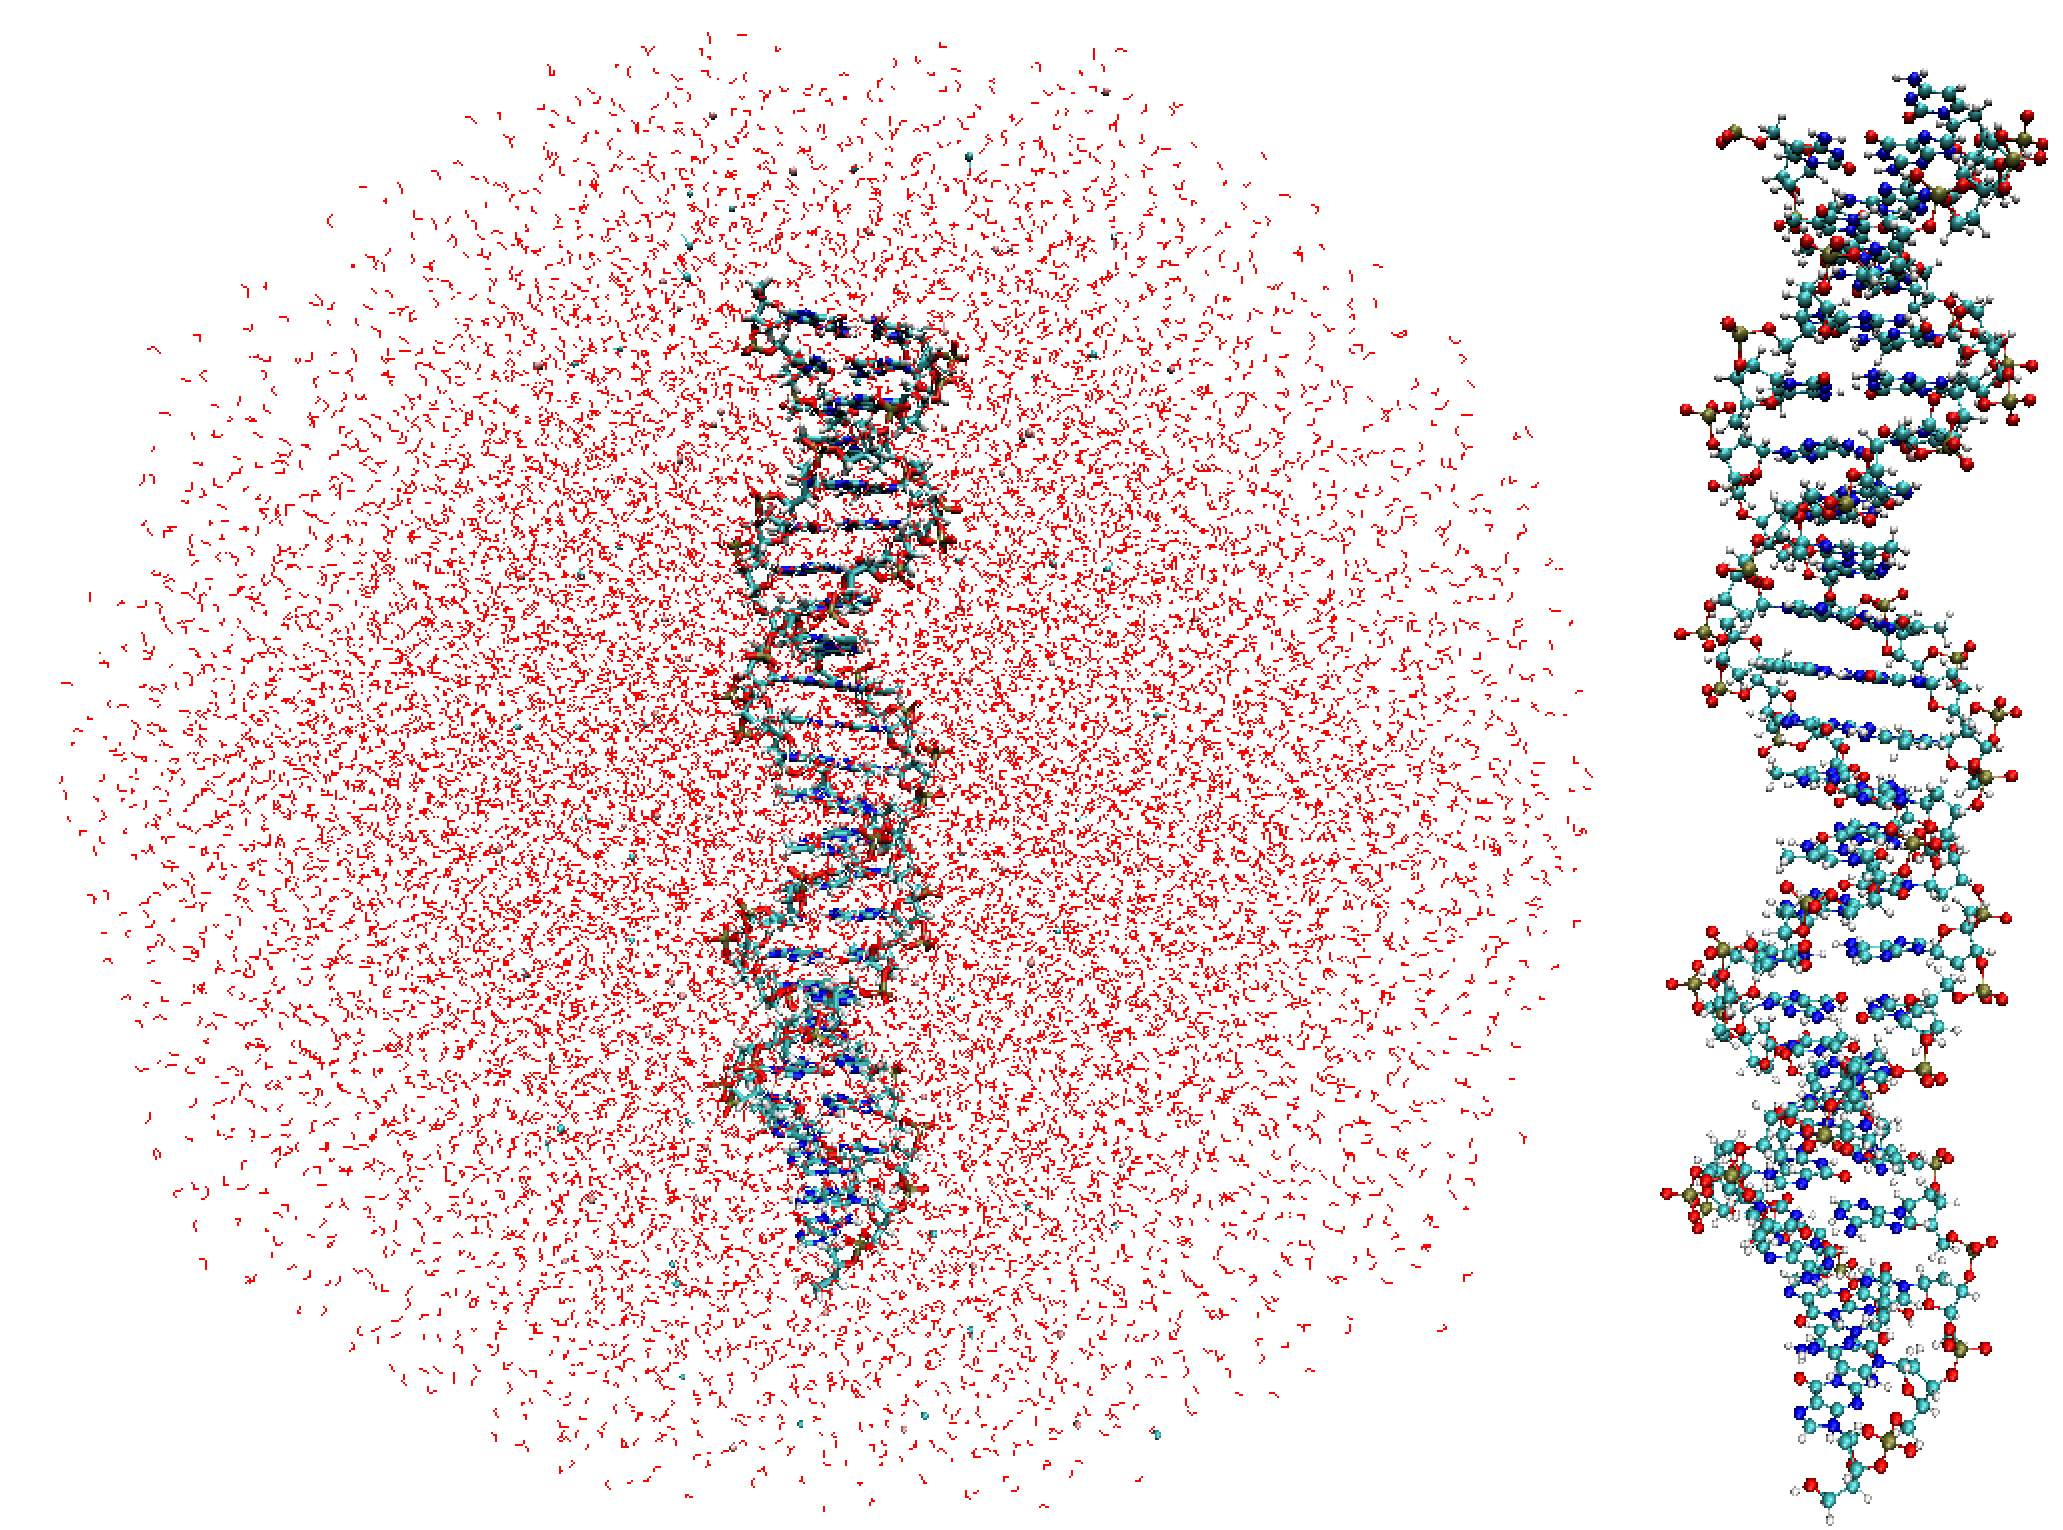
\includegraphics[scale=.165]{images/sample_img.png}
\caption{A typical snapshot of the molecular dynamics simulation setup of a 24mer dsDNA. On the left, the dsDNA molecule and ions are solvated in water and on the right, a snapshot of dsDNA.}
\label{c3:fig1}
\end{center}
\end{figure}

\section{Simulation details}\label{c3:s2}
The initial structure of a given sequence has been generated using NAB in AMBERTOOLS 18~\cite{amber}.
We have used Arnott right-handed B-DNA fiber parameters~\cite{arnott} and Arnott right-handed A-RNA fiber parameters~\cite{arnottrna} for DNA and RNA strands, respectively.
Furthermore, to obtain the initial geometry of DRH, we have first generated an A-form RNA (i.e., start with pure A-form) and then modified all Uracil to Thymine and changed the sugar molecule from ribose to deoxyribose (i.e., replace the OH group at 2$^\prime$ with an H) in one of the strands.
Then, in the first few nanoseconds of production run, we observed that the molecule changes its geometry to a mixed A-B form.
Our analysis has ignored the first 100 nanoseconds of the production simulation.
Lastly, to methylate or hydroxymethylate the desired cytosine in the structure, we have modified the initial structures obtained from NAB using the leap program in AMBERTOOLS 18. \clearpage

To describe the DNA and RNA strands in the MD simulations, we have used the PARMBSC1~\cite{parmbsc1} and OL3 forcefield corrections~\cite{zgarbova2011refinement}, respectively along with PARMBSC0~\cite{perez2007refinement} and parm99 force field~\cite{cheatham1999modified}.
Furthermore, we have used additional parameters for methylated and hydroxymethylated cytosine~\cite{battistini2021impact,perez2012impact}.
For each sequence, once the initial dsNA structure was generated, the molecule was solvated in a truncated octahedral water box of explicit TIP3P water molecules~\cite{tip3p} with a water layer of a minimum 10 \AA \ surrounding the dsNA molecule. 
Subsequently, the solvated dsNA was neutralized with K$^+$ ions, and then K$^+$ and Cl$^-$ ion-pairs were added to make the salt concentration approximately 150 mM.
The ions were described using the Joung and Cheatham model~\cite{jcion} and added with the constraint that the ions are at least 5 \AA \ away from the dsNA molecule and at least 3.5 \AA \ away from each other.
For training sequences in libraries (\cref{palinold,epilib}), this complete initial setup contains $\approx$ 45,000 atoms, of which $\approx$ 40,000 are from water molecules.
A typical snapshot of such an initial system is shown in \cref{c3:fig1}. 
The system size is smaller for the sequences in the 12mer library (\cref{endlib}).

The system preparation is followed by an energy minimization step to minimize the solvent energy.
Then the system temperature is slowly raised to 300 K, followed by an equilibration step of 50 picoseconds.
All simulations were performed using AMBER 18 modules~\cite{amber}.
Simulations were carried out in the NPT ensemble using the Berendsen algorithm~\cite{npt} to maintain the temperature (at 300K) and the pressure (1 atm) with a coupling constant of 5 picoseconds.
Furthermore, we have used SHAKE~\cite{shake} algorithm to freeze the motion of bonds involving Hydrogen allowing a larger simulation time-step of 2 femtoseconds.
Simulations were carried out under periodic boundary conditions, and long-range electrostatic interactions were treated using the particle mesh Ewald method~\cite{pme} with 9 \AA \ real space cut-off.
The short-range Lennard-Jones interactions were also truncated at 9 \AA.
Note that most simulation parameters have been motivated by the choices made by the Ascona B-DNA Consortium (ABC)~\cite{lavery2010systematic}.
Finally, for each system, 10 $\mu$s of production run simulations were carried out at EPFL HPC facilities using GPUs with each node containing 2 Xeon-Gold processors and 2 NVIDIA V100 PCIe 32 GB GPUs.
Production run simulation trajectories were stored at two picosecond intervals.
Each production run simulation of length 10 $\mu$s took approximately two months for a 24mer.
\section{Training library}\label{c3:s3}
In this section, we have discussed the various training and test sequences that are used to train the cgNA$+$ model parameter sets.
\subsection{Training library for interior blocks and GC ends of dsNA parameter sets}
We have simulated a comprehensive set of palindromic sequences to train the parameter sets for dsDNA and dsRNA called the palindromic training library, originally proposed in ref.~\cite{patelithesis}.
It contains 16 training sequences (with GC ends) of length 24 base-pairs such that the library has almost similar instances for all monomers, dimers, and trimer, and all 256 tetramers appear at least once on both strands.
The sequences in both libraries, \Lbdna \ and \Lbrna \ are provided in \cref{palinold}.
The palindromic nature of these training libraries allows quantifying the convergence of MD simulations, which is otherwise non-trivial as discussed in \cref{c3:s5}. \hfill \clearpage

\begin{table}[H]
\begin{center}
\begin{tabular}{ c || c | c | c  | c | c }
Sequence index & \multicolumn{5}{c}{Acceptance rate}\\
\hline    
   &\Lbdna & \Lbrna & \Lbdrh & \Lbm & \Lbh \\ 
\hline    
1  & 85.29 & 77.51 & 78.78 & 83.25 & 86.39 \\
2  & 83.10 & 76.27 & 74.31 & 85.90 & 83.52 \\
3  & 86.61 & 80.78 & 81.57 & 84.28 & 86.71 \\
4  & 85.00 & 74.41 & 78.69 & 86.18 & 84.07 \\
5  & 82.90 & 80.32 & 80.19 & 86.11 & 87.74 \\
6  & 88.83 & 84.37 & 78.24 & 87.93 & 87.08 \\
7  & 84.40 & 74.86 & 75.46 & 88.44 & 85.16 \\
8  & 85.24 & 78.40 & 80.72 & 82.89 & 84.10 \\
9  & 79.94 & 76.77 & 71.90 & 74.86 & 87.44 \\
10 & 88.97 & 75.89 & 75.24 & 88.30 & 84.69 \\
11 & 84.29 & 80.03 & 74.41 & 83.20 & 82.67 \\
12 & 82.15 & 82.94 & 76.74 & 91.40 & 89.72 \\
13 & 88.47 & 78.89 & 79.60 \\
14 & 88.86 & 76.92 & 80.99 \\
15 & 79.58 & 81.24 & 75.65 \\
16 & 82.46 & 83.00 & 81.37 \\
\end{tabular}
\end{center}
\caption{
\% MD snapshots left after discarding snapshots with broken H-bonds.  The total number of configurations before filtering is $10\cdot5\cdot10^5$ ($10~\mu s$) for each training sequence listed in 
%\cref{chapter}{appendix}
\cref{palinold,epilib}.
}
\label{c3:accept_tab_int}
\end{table}

\begin{table}[ht!]
\small
\centering
\begin{tabular}{c||c|c||c|c||c|c||c}
 Sequence   & Acceptance & Sequence   & Acceptance & Sequence   & Acceptance & Sequence   & Acceptance \\
  index  & rate & index & rate & index & rate & index & rate \\
\hline
  1  &  24.49  & 2  & 27.86 & 3  & 29.72 &  4  & 30.13 \\
  5  &  28.33  & 6  & 32.89 & 7  & 30.02 &  8  & 32.96 \\
  9  &  17.53  & 10 & 28.93 & 11 & 28.20 &  12 & 29.07 \\
  13 &  35.47  & 14 & 25.39 & 15 & 28.96 &  16 & 35.76 \\
  17 &  19.90  & 18 & 24.30 & 19 & 16.33 &  20 & 24.91 \\
  21 &  24.17  & 22 & 30.86 & 23 & 13.62 &  24 & 29.54 \\
  25 &  33.59  & 26 & 31.29 & 27 & 21.46 &  28 & 38.57 \\
  29 &  27.02  & 30 & 29.85 & 31 & 23.71 &  32 & 25.38 \\
  33 &  61.08  & 34 & 59.17 & 35 & 66.19 &  36 & 62.76 \\
  37 &  57.17  & 38 & 65.35 & 39 & 49.92 &  40 & 62.90 \\
  41 &  54.78  & 42 & 53.06 & 43 & 71.07 &  44 & 66.19 \\
  45 &  39.36  & 46 & 43.43 & 47 & 54.22 &  48 & 46.07 \\
  49 &  64.36  & 50 & 65.49 & 51 & 67.62 &  52 & 60.02 \\
  53 &  64.96  & 54 & 64.26 & 55 & 49.42 &  56 & 68.65 \\
  57 &  58.70  & 58 & 61.25 & 59 & 52.68 &  60 & 59.07 \\
\end{tabular}
\caption{\% MD snapshots left after discarding snapshots with broken H-bonds. 
The total number of configurations before filtering is $3\cdot5\cdot10^5$ ($3~\mu s$) for each sequence listed in \cref{endlib}.}
\label{c3:accept_tab_end}
\end{table} \clearpage

\noindent Using these training sequences with GC ends, we have estimated model parameters for interior blocks and GC ends.
Along with the training sequences, \Lbdna \ and \Lbrna \  also contain test sequences comprising a random palindrome, some mechanically exceptional sequences such as poly(A), poly(AT), sequences with point mutations and A-tracts. 
We have used the same training library (as dsDNA or dsRNA) to train coarse-grain parameters for DRH, but the sequences are not palindrome anymore.
More details on the parameter sets are provided in \cref{c4:subsec_prm}. 

\subsection{Training library for dsDNA non-GC ends parameters}
Furthermore, we have used an additional 60 sequences of length 12 base-pairs (refer \cref{endlib}) to train parameters for non-GC ends. 
For each non-GC end, we have four sequences starting with the non-GC end (while another end is GC) followed by one of the RR, RY, YR, and YY steps (where R represents the purine base and Y represents the pyrimidine base) for a diverse training set, and the rest of the sequence is chosen randomly.
Thus, to train model parameters for a given non-GC end, we have MD time-series data from four sequences with a non-GC end followed by different contexts.
For each sequence in the end library (\Lbe), we have generated an MD time-series of $3~\mu$s.
More details on how these libraries are used to calculate coarse-grained model parameters are provided in \cref{c2:sec4}.

\subsection{Training library for epigenetically modified}
In this work, the objective is to obtain a parameter set that allows epigenetically modified \cpg steps, in particular, methylated or hydroxymethylated, which can be symmetric or asymmetric.
For training such parameters for modified \cpg steps, we have again designed a palindromic training library that contains symmetrically and asymmetrically modified \cpg steps in diverse sequence contexts, as well as modified steps next to each other. 
The libraries are referred to as \Lbm \ and \Lbh \ for training sequences containing methylated and hydroxymethylated \cpg steps, respectively, and details are provided in \cref{epilib}.
Moreover, \cref{epilib} also contains a few test sequences, in particular, typical \cpg islands with \cpg step modifications.

\section{MD data processing}\label{c3:s4}
As described earlier in \cref{c3:s2} for each sequence (except the sequences in \Lbe), we have run 10 $\mu$s of the production run. 
The data are stored in binary format (.nc) provided by AMBER, and it takes $\approx 3.3$ TB and $\approx 96$ GB of storage to save the data for one sequence with water and without water, respectively.
The first step after the production run is to strip the water using CPPTRAJ~\cite{roe2013ptraj,roe2018parallelization}
which makes further analysis easier due to the smaller size of the trajectories.
Subsequently, we fit the frames in the MD trajectories, compute the cgNA$+$ model internal coordinates from frames and discard snapshots with broken H-bonds.
The last step is to compute the first and second moments, i.e., oligomer level Gaussian statistics (refer \cref{c2:eq_moments}) for the internal coordinates distributions in (filtered) MD time-series for each sequence.

H-bond filtering is one of the most crucial steps in MD analysis, and in \cref{c3:accept_tab_int,c3:accept_tab_end}, we have provided the \% of accepted snapshots for each training sequence in various training libraries along with the total number of snapshots.
For each sequence with GC ends used for the training of interior block parameters, the acceptance is $\approx 70-90\%$.
In contrast, the acceptance after H-bond filtering in the training sequences for end-block parameters is comparatively lower, i.e., $\approx 18-71 \%$ and highly depends on its non-GC end.
A similar acceptance of MD snapshots is observed for the test sequences; therefore, details of those sequences are omitted for brevity.

In \cref{c3:fig_hist_filter1,c3:fig_hist_filter2,c3:fig_hist_filter3,c3:fig_hist_filter4}, we have plotted marginal normalized histograms for various internal coordinates observed in MD time series before and after H-bond filtering for sequence index 1 in \Lbdna. 
The histograms are plotted for the half-sequence while reading the sequence from both the Crick and Watson strands.
The primary objective of the plots is to visualize the effect of H-bond filtering in the MD data (by comparing histograms in dotted and solid lines for MD data before and after filtering, respectively). 
Moreover, since the sequence is palindromic, the two dotted histograms corresponding to reads from the Crick and the Watson strand comment on the convergence of MD simulations (details are provided in \cref{c2:s5sb1,c3:s5}).

Notably, for all internal coordinates, the two histograms in dotted and solid lines for broken H-bond filtered and unfiltered MD data, respectively, are indistinguishable except for intra-translational coordinates (Shear, Stretch, and Stagger) for terminal G and phosphate rotational parameters for the terminal base-pair step GC on both Crick and Watson strands. 
It highlights that the rejected MD snapshots with broken H-bond are primarily due to fraying of terminal base-pairs and do not affect the distribution of coordinates for internal base-pairs and base-pair steps.
We observed similar patterns for other sequences in \Lbdna \ and other dsNA libraries.

\section{Convergence of MD simulations}\label{c3:s5}
How to determine whether a simulation is long enough is a 
challenging task? 
Several studies have investigated the convergence of MD simulations.
Traditionally, the decay of the average root mean square deviation values from some reference structure over time has been used to assess the convergence of MD simulations.
Alternatively, one can run multiple production runs starting from different initial configurations and compare statistics for those independent trajectories.
In particular, for dsDNA (ignoring terminal base-pairs), it has been suggested that 
1-5 $\mu$s of MD simulations are sufficient for converging its structure and dynamics~\cite{galindo2015convergence}. 
In this work, to quantify the convergence of MD time series, we have exploited the palindromic nature of dsNA sequences and defined the palindromic error ($\er_{\text{KL}}^{\text{palin}}$) as the symmetric Kullback-Leibler divergence between Gaussian pdfs while reading the dsNA sequence from the Crick and Watson strands. 
The shape contribution in the palindromic error is the Mahalanobis distance denoted as $\er_{\M}^{\text{palin}}$. 
More details on these computations are provided in \cref{c2:s5sb1}.   

Firstly, in \cref{c3:fig_hist_filter1,c3:fig_hist_filter2,c3:fig_hist_filter3,c3:fig_hist_filter4}, each panel has two marginal normalized histograms (in solid line) for various internal coordinates observed in the MD time series while reading the sequence from the Crick and Watson strands.
The deviations in the two histograms (plotted in the same solid color) highlight the convergence error, and it is evident from the plots that the two solid plots are on top of each other for intra and inter variables. In the case of phosphate coordinates, one can find examples of observing two solid lines, for example, WRot and WTra coordinates for AA ([3,2] panel). In general, it can be observed that the phosphate coordinates are slightly less converged than the base coordinates, which is consistent with the earlier observations~\cite{patelithesis}. \clearpage

\begin{figure}
\begin{center}
\subfloat{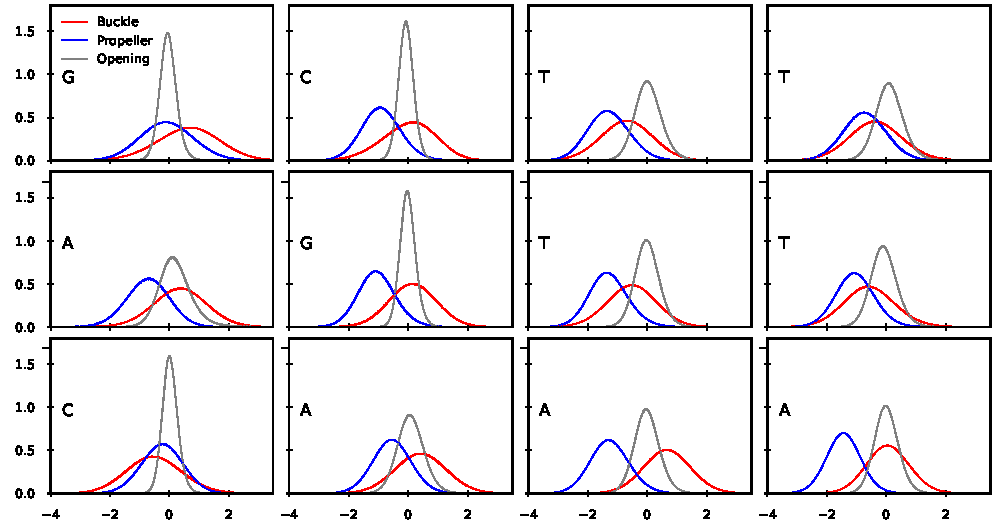
\includegraphics[scale=0.9]{./images/DNA-unfiltintra-r-seq-1.pdf} }\\
\subfloat{
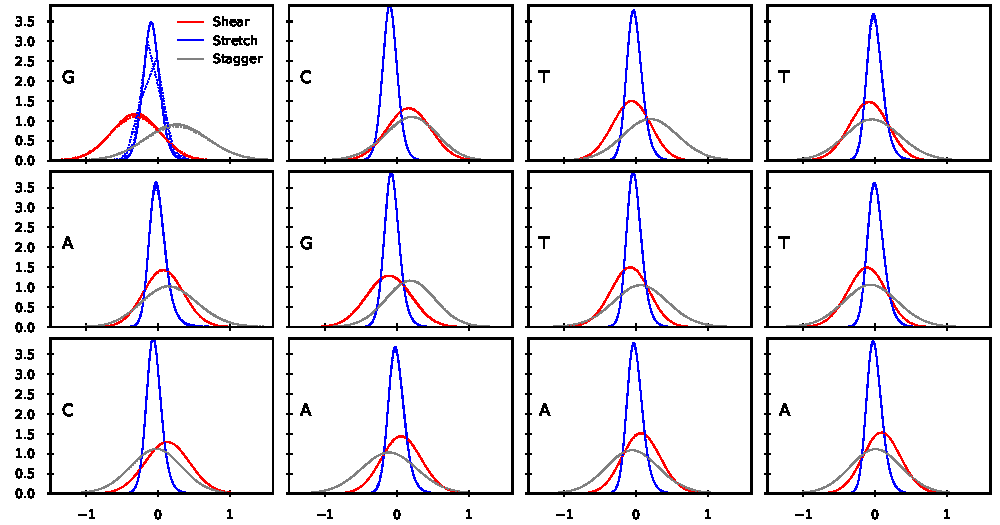
\includegraphics[scale=0.9]{./images/DNA-unfiltintra-t-seq-1.pdf}} \\
\end{center}
\caption{Marginal normalized histograms for intra base-pair rotational (top figure) and translational (bottom figure) coordinates for sequence index 1 in \Lbdna.
The coordinates are plotted from left to right and from top to bottom for base-pairs 1 to 12 while reading the strands from both Crick and Watson strands. 
The histograms in solid and dotted lines are for filtered (snapshots without broken H-bonds) and unfiltered MD data, respectively.
}
\label{c3:fig_hist_filter1}
\end{figure} \clearpage

\begin{figure}
\begin{center}
\subfloat{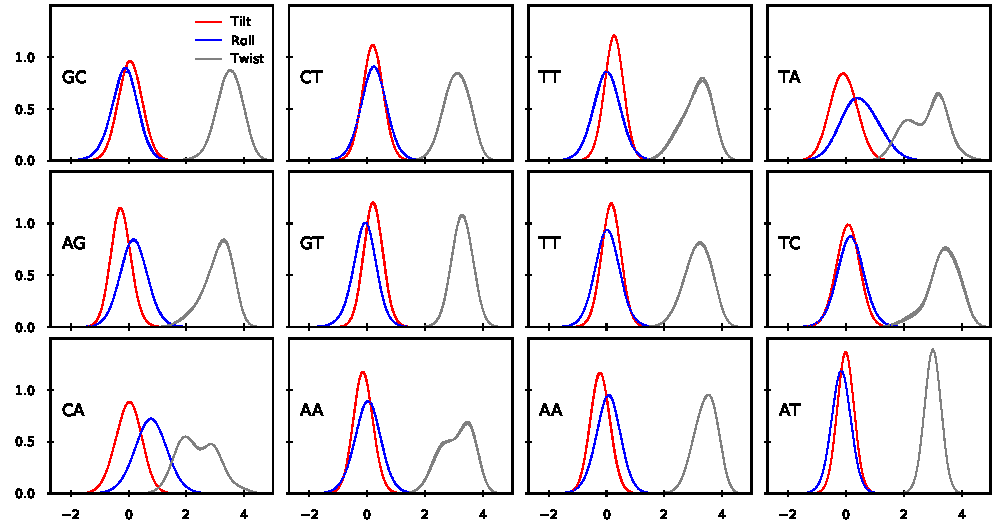
\includegraphics[scale=0.9]{./images/DNA-unfiltinter-r-seq-1.pdf} }\\
\subfloat{
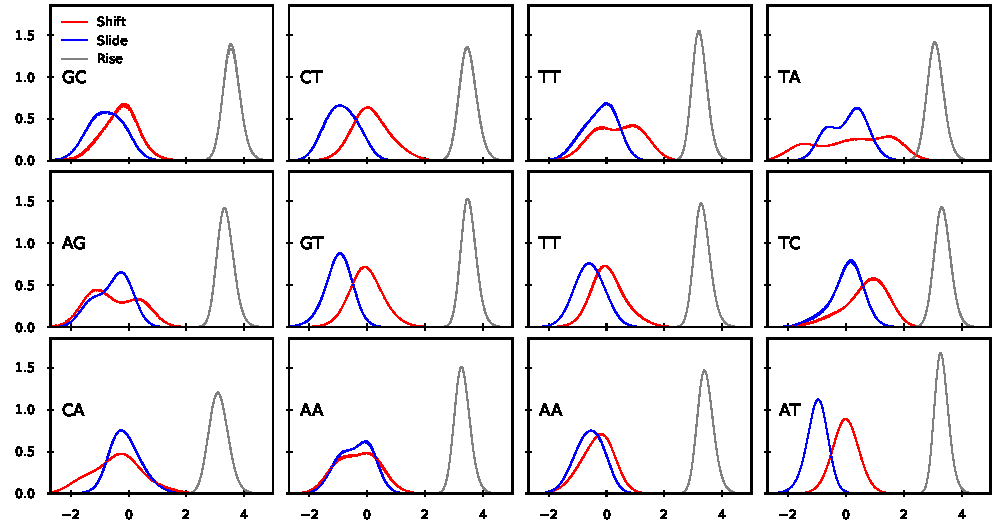
\includegraphics[scale=0.9]{./images/DNA-unfiltinter-t-seq-1.pdf}} \\
\end{center}
\caption{Marginal normalized histograms for inter base-pair rotational (top figure) and translational (bottom figure) coordinates for sequence index 1 in \Lbdna.
The coordinates are plotted from left to right and from top to bottom for base-pair steps 1 to 12 while reading the strands from both Crick and Watson strands.  
The histograms in solid and dotted lines are for filtered (snapshots without broken H-bonds) and unfiltered MD data, respectively.
}
\label{c3:fig_hist_filter2}
\end{figure} \clearpage

\begin{figure}
\begin{center}
\subfloat{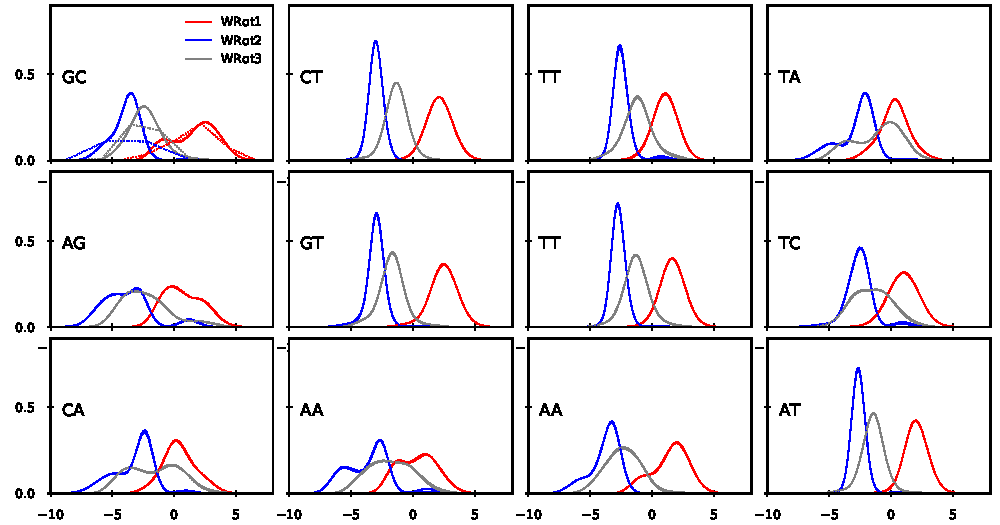
\includegraphics[scale=0.9]{./images/DNA-unfiltphosW-r-seq-1.pdf} }\\
\subfloat{
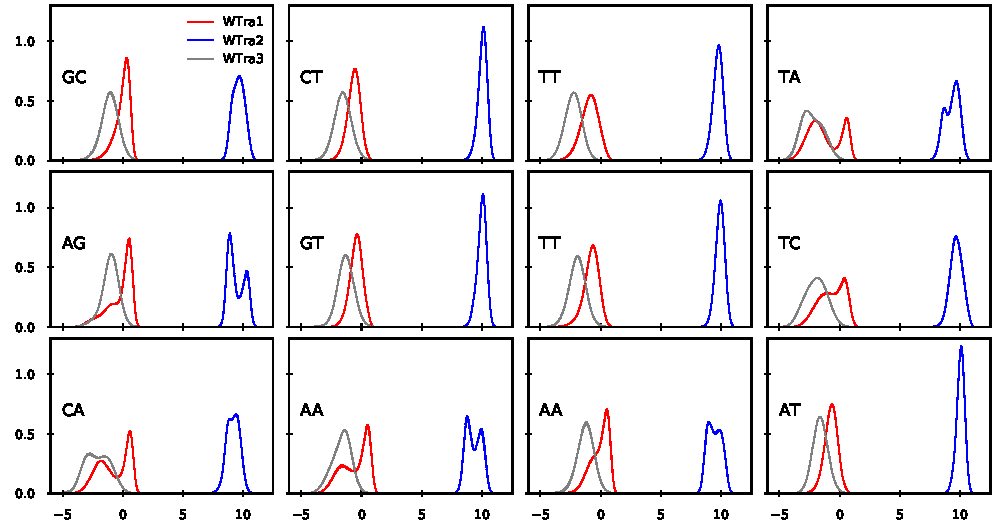
\includegraphics[scale=0.9]{./images/DNA-unfiltphosW-t-seq-1.pdf}} \\
\end{center}
\caption{Marginal normalized histograms for Watson phosphate rotational (top figure) and translational (bottom figure) coordinates for sequence index 1 in \Lbdna. The coordinates are plotted from left to right and from top to bottom for base-pair steps 1 to 12 while reading the strands from both Crick and Watson strands. 
The histograms in solid and dotted lines are for filtered (snapshots without broken H-bonds) and unfiltered MD data, respectively.
}
\label{c3:fig_hist_filter3}
\end{figure}\clearpage

\begin{figure}
\begin{center}
\subfloat{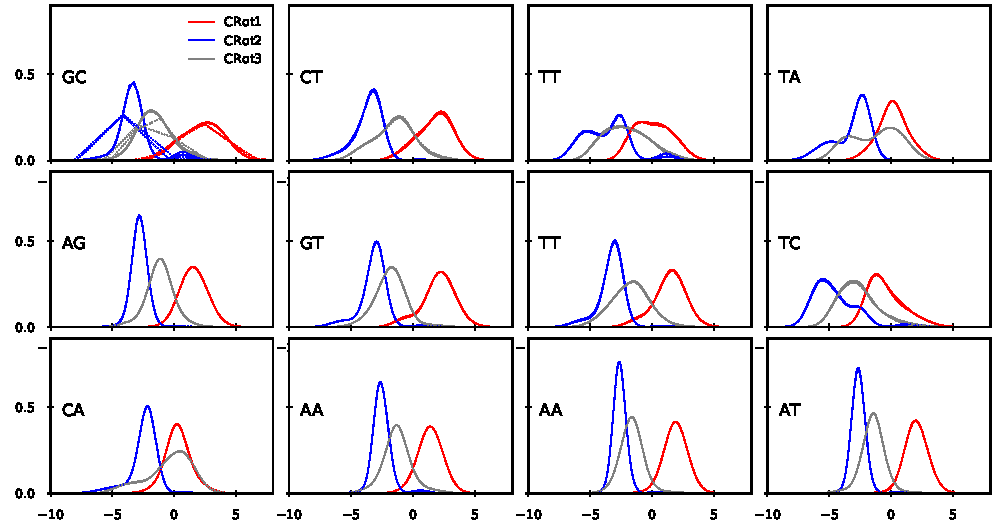
\includegraphics[scale=0.9]{./images/DNA-unfiltphosC-r-seq-1.pdf} }\\
\subfloat{
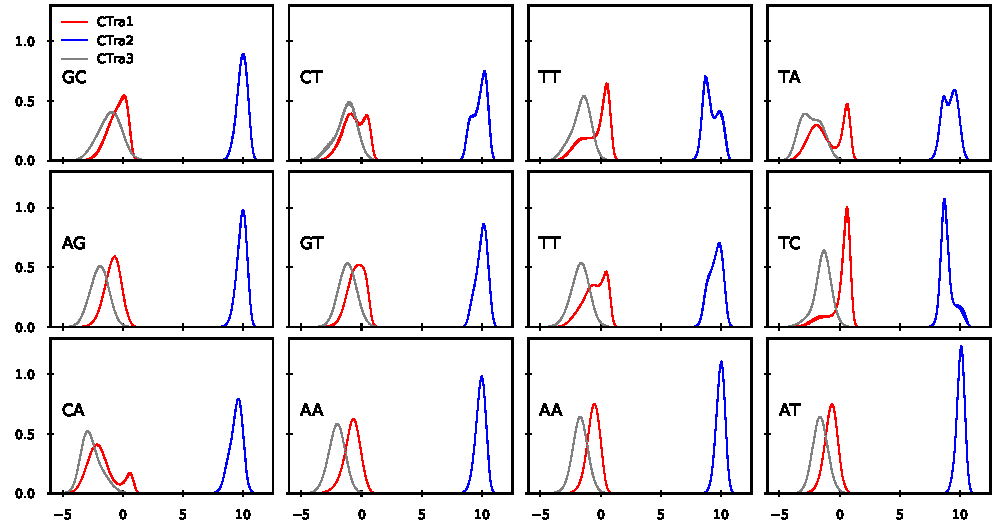
\includegraphics[scale=0.9]{./images/DNA-unfiltphosC-t-seq-1.pdf}} \\
\end{center}
\caption{Marginal normalized histograms for Crick phosphate rotational (top figure) and translational (bottom figure) coordinates for sequence index 1 in \Lbdna. The coordinates are plotted from left to right and from top to bottom for base-pair steps 1 to 12 while reading the strands from both Crick and Watson strands. 
The histograms in solid and dotted lines are for filtered (snapshots without broken H-bonds) and unfiltered MD data, respectively.
}
\label{c3:fig_hist_filter4}
\end{figure}\clearpage


In \cref{c3:tab_con_dna}, we have provided $\er_{\text{KL}}^{\text{palin}}$ and  $\er_{\M}^{\text{palin}}$ per degree of freedom (dof) for the training sequences in \Lbdna \ over the simulation time.
The dof is the number of internal coordinates required to describe the configuration of a given dsDNA sequence, i.e., for a sequence of length $N$ base-pairs, the dofs are $24N-18$.
Note that we have also included one test sequence (index 17) with 20 $\mu$s simulation data.  
In \cref{c3:tab_con_dna}, it can be observed that a) different sequences converge differently, for example, the convergence error (both $\er_{\text{KL}}^{\text{palin}}$ and $\er_{\M}^{\text{palin}}$) in sequence index 10 is almost double that of 11, and b) with longer simulation times, the convergence error decreases for all sequences. 
Here, we have provided the convergence error for 1-10 $\mu$s simulation time. 
Notably, after $\approx 5 \ \mu$s simulation time, the decrease in convergence error is relatively tiny.
Moreover, for sequence index 17, we have generated 20 $\mu$s of MD time-series. Although the convergence error decreases for $20 \ \mu$s simulation data from $10 \mu$s, it is still comparable to the convergence error in other training sequences. 
Lastly, the average of $\er_{\text{KL}}^{\text{palin}}$ for $10 \ \mu$s data for all training sequences is 0.0050 which is very small, as can be seen in \cref{c2:KL_envelope}.
The corresponding $\er_{\M}^{\text{palin, avg}}$ is 0.0009 which can be considered equal to 0.03 \AA \ or rad/5 per dof which is tiny.

Furthermore, to set a \textit{scale} for this convergence error, we have computed the average pair-wise symmetric KL divergence and symmetric Mahalanobis distance between the training sequences in \Lbdna \ (as described in \cref{c2:s5sb4}), which is 0.4395 and 0.0245 per dof, respectively.
It sets a \textit{scale} quantifying the average difference in various sequences in the training library, i.e., quantifies variation over sequence.
This \textit{scale} is approximately 27 and 88 times larger than $\er_{\M}^{\text{palin}}$  and  $\er_{\text{KL}}^{\text{palin}}$ observed for $10 \ \mu$s data. 
Thus, we conclude that $10 \ \mu$s of the MD simulations are well converged and sufficient to train the cgNA$+$ model.
%  0.0211  &  0.3378 --- MDNA %  0.0214  &  0.3449  --- HDNA

Moreover, we again observed that convergence trends are very similar for all palindromic sequences in \Lbrna, \Lbm, and \Lbh \ and therefore, for brevity, we have provided the average of convergence statistics for training sequences in the various libraries. In \cref{c3:tab_con_rest}, we have provided the average of $\er_{\text{KL}}^{\text{palin}}$ and $\er_{\M}^{\text{palin}}$ taken over for all the training sequences in \Lbrna, \Lbm, and \Lbh \ and corresponding \textit{scales}.
Firstly, the convergence trends in \Lbm \ and \Lbm \ are very similar to the trends in \Lbdna, which can be expected as the two libraries differ from \Lbdna \ slightly in terms of epigenetic modifications in some of the bases.
Similarly, the \textit{scales} in the two libraries are comparable to the \textit{scale} in \Lbdna. 
In contrast, dsRNA sequences appear to converge with a palindromic error similar to that observed in dsDNA, but in a relatively shorter simulation time, and after that, the palindromic error decreases very slowly.  
It might be attributed to the smaller conformational space of dsRNA compared to dsDNA~\cite{noy2004relative,noy2005structure}.

Lastly, DRH sequences are not palindromes, and therefore, we can not use palindromic error to quantify the convergence in the MD simulations of DRH. 
As mentioned earlier, we have generated 10 $\mu$s of simulation data for each sequence, which are essentially two independent trajectories of 5 $\mu$s started with two different random initial configurations. 
Therefore, for DRH sequences, we have compared the statistics for these two independent trajectories, which are extremely close and, thus, concluded that the time-series are sufficiently converged.
\clearpage

\begin{sidewaystable}[ht]
\begin{center}
\begin{footnotesize}
\begin{tabular}{| c | c c c c c c c c c c c c c c c c | c | }
\hline
Index & 1 & 2 & 3 & 4 & 5 & 6 & 7 & 8 & 9 & 10 & 11 & 12 & 13 & 14 & 15 & 16 & 17 \\ \hline
& & & & & & & $\er_{\M}^{\text{palin}}$ & & & & & & & & & & \\ \hline
1  $\mu$s & 0.0041 & 0.0049 & 0.0040 & 0.0030 & 0.0033 & 0.0076 & 0.0016 & 0.0045 & 0.0024 & 0.0034 & 0.0031 & 0.0084 & 0.0031 & 0.0045 & 0.0072 & 0.0016 & 0.0037 \\ \hline
2  $\mu$s & 0.0021 & 0.0028 & 0.0028 & 0.0022 & 0.0020 & 0.0027 & 0.0017 & 0.0022 & 0.0025 & 0.0014 & 0.0020 & 0.0033 & 0.0028 & 0.0030 & 0.0037 & 0.0014 & 0.0025 \\ \hline
3  $\mu$s & 0.0016 & 0.0018 & 0.0018 & 0.0014 & 0.0015 & 0.0018 & 0.0010 & 0.0014 & 0.0015 & 0.0013 & 0.0016 & 0.0029 & 0.0016 & 0.0017 & 0.0030 & 0.0013 & 0.0022 \\ \hline
4  $\mu$s & 0.0014 & 0.0014 & 0.0016 & 0.0013 & 0.0012 & 0.0014 & 0.0011 & 0.0012 & 0.0012 & 0.0013 & 0.0012 & 0.0021 & 0.0015 & 0.0017 & 0.0023 & 0.0011 & 0.0026 \\ \hline
5  $\mu$s & 0.0013 & 0.0012 & 0.0015 & 0.0009 & 0.0012 & 0.0012 & 0.0012 & 0.0012 & 0.0014 & 0.0011 & 0.0011 & 0.0020 & 0.0014 & 0.0015 & 0.0020 & 0.0011 & 0.0026 \\ \hline
6  $\mu$s & 0.0012 & 0.0010 & 0.0013 & 0.0009 & 0.0010 & 0.0011 & 0.0009 & 0.0011 & 0.0010 & 0.0012 & 0.0009 & 0.0015 & 0.0011 & 0.0012 & 0.0018 & 0.0009 & 0.0021 \\ \hline
7  $\mu$s & 0.0011 & 0.0010 & 0.0012 & 0.0009 & 0.0013 & 0.0011 & 0.0009 & 0.0010 & 0.0009 & 0.0013 & 0.0009 & 0.0012 & 0.0010 & 0.0011 & 0.0018 & 0.0007 & 0.0019 \\ \hline
8  $\mu$s & 0.0011 & 0.0009 & 0.0010 & 0.0008 & 0.0010 & 0.0009 & 0.0008 & 0.0011 & 0.0008 & 0.0013 & 0.0008 & 0.0010 & 0.0009 & 0.0010 & 0.0019 & 0.0007 & 0.0017 \\ \hline
9  $\mu$s & 0.0011 & 0.0009 & 0.0010 & 0.0007 & 0.0009 & 0.0008 & 0.0009 & 0.0011 & 0.0008 & 0.0014 & 0.0007 & 0.0009 & 0.0008 & 0.0009 & 0.0017 & 0.0007 & 0.0016 \\ \hline
10 $\mu$s & 0.0009 & 0.0009 & 0.0010 & 0.0007 & 0.0009 & 0.0008 & 0.0008 & 0.0011 & 0.0008 & 0.0012 & 0.0006 & 0.0009 & 0.0008 & 0.0009 & 0.0014 & 0.0007 & 0.0015 \\ \hline
20 $\mu$s & & & & & & & & & & & & & & & & & 0.0008 \\ \hline
& & & & & & & $\er_{\text{KL}}^{\text{palin}}$ & & & & & & & & & & \\ \hline
1  $\mu$s & 0.0570 & 0.0634 & 0.0560 & 0.0445 & 0.0402 & 0.0849 & 0.0211 & 0.0532 & 0.0342 & 0.0470 & 0.0363 & 0.1102 & 0.0426 & 0.0684 & 0.1076 & 0.0239 & 0.0420 \\ \hline
2  $\mu$s & 0.0213 & 0.0318 & 0.0354 & 0.0259 & 0.0254 & 0.0299 & 0.0192 & 0.0261 & 0.0235 & 0.0139 & 0.0149 & 0.0286 & 0.0311 & 0.0383 & 0.0419 & 0.0144 & 0.0221 \\ \hline
3  $\mu$s & 0.0118 & 0.0153 & 0.0199 & 0.0129 & 0.0147 & 0.0169 & 0.0092 & 0.0142 & 0.0148 & 0.0112 & 0.0138 & 0.0227 & 0.0165 & 0.0166 & 0.0271 & 0.0116 & 0.0178 \\ \hline
4  $\mu$s & 0.0084 & 0.0110 & 0.0140 & 0.0112 & 0.0111 & 0.0102 & 0.0094 & 0.0113 & 0.0092 & 0.0080 & 0.0099 & 0.0146 & 0.0142 & 0.0137 & 0.0162 & 0.0083 & 0.0238 \\ \hline
5  $\mu$s & 0.0085 & 0.0087 & 0.0114 & 0.0070 & 0.0096 & 0.0100 & 0.0091 & 0.0096 & 0.0091 & 0.0070 & 0.0080 & 0.0126 & 0.0144 & 0.0125 & 0.0126 & 0.0065 & 0.0221 \\ \hline
6  $\mu$s & 0.0078 & 0.0080 & 0.0120 & 0.0061 & 0.0082 & 0.0100 & 0.0066 & 0.0085 & 0.0061 & 0.0070 & 0.0063 & 0.0099 & 0.0090 & 0.0079 & 0.0105 & 0.0048 & 0.0176 \\ \hline
7  $\mu$s & 0.0072 & 0.0068 & 0.0102 & 0.0056 & 0.0083 & 0.0077 & 0.0058 & 0.0071 & 0.0059 & 0.0074 & 0.0065 & 0.0072 & 0.0084 & 0.0068 & 0.0102 & 0.0040 & 0.0148 \\ \hline
8  $\mu$s & 0.0076 & 0.0057 & 0.0082 & 0.0047 & 0.0062 & 0.0063 & 0.0050 & 0.0074 & 0.0049 & 0.0072 & 0.0050 & 0.0058 & 0.0069 & 0.0058 & 0.0103 & 0.0037 & 0.0118 \\ \hline
9  $\mu$s & 0.0070 & 0.0056 & 0.0070 & 0.0042 & 0.0051 & 0.0045 & 0.0051 & 0.0068 & 0.0050 & 0.0079 & 0.0041 & 0.0049 & 0.0056 & 0.0055 & 0.0095 & 0.0035 & 0.0107 \\ \hline
10 $\mu$s & 0.0055 & 0.0052 & 0.0065 & 0.0037 & 0.0048 & 0.0041 & 0.0042 & 0.0063 & 0.0050 & 0.0062 & 0.0033 & 0.0046 & 0.0052 & 0.0051 & 0.0072 & 0.0032 & 0.0092 \\ \hline
20 $\mu$s & & & & & & & & & & & & & & & & & 0.0035 \\ \hline
\end{tabular}
\end{footnotesize}
\end{center}
\caption{Palindromic error, $\er_{\text{KL}}^{\text{palin}}$ and Mahalanobis error, $\er_{\M}^{\text{palin}}$ per dof for the sequences in the training sequences for cgDNA$+$ model and a test palindrome sequence. The details of the sequences are in \cref{palinold}.
}
\label{c3:tab_con_dna}
\end{sidewaystable} \clearpage

\begin{table}[H]
\begin{center}
\begin{small}
%\begin{tabular}{| c | p{0.45cm} p{0.45cm} p{0.45cm} p{0.45cm}  p{0.45cm} p{0.45cm} p{0.45cm} p{0.45cm}  p{0.45cm} p{0.45cm} p{0.45cm} p{0.45cm}  p{0.45cm} p{0.45cm} p{0.45cm} p{0.6cm} | p{0.6cm} | }
\begin{tabular}{ c || c c | c c | c c}
& \multicolumn{2}{c}{\Lbrna} & \multicolumn{2}{c}{\Lbm} & \multicolumn{2}{c}{\Lbh} \\
\hline
 Simulation & \multirow{2}{*}{$\er_{\M, \ \text{avg}}^{\text{palin}}$} & \multirow{2}{*}{$\er_{\text{KL,  avg}}^{\text{palin}}$} & \multirow{2}{*}{$\er_{\M, \ \text{avg}}^{\text{palin}}$} & \multirow{2}{*}{$\er_{\text{KL, avg}}^{\text{palin}}$} & \multirow{2}{*}{$\er_{\M, \ \text{avg}}^{\text{palin}}$} & \multirow{2}{*}{$\er_{\text{KL, avg}}^{\text{palin}}$} \\
time ($\mu$s) & & & & & & \\
\hline
0.25  & 0.0010 & 0.0118 & & & & \\
0.50  & 0.0008 & 0.0076 & & & & \\
0.75  & 0.0008 & 0.0071 & & & & \\
1     & 0.0007 & 0.0061 & 0.0036 & 0.0492 & 0.0035 & 0.0457 \\
2     & 0.0008 & 0.0068 & 0.0022 & 0.0245 & 0.0022 & 0.0231 \\
3     & 0.0008 & 0.0063 & 0.0017 & 0.0156 & 0.0017 & 0.0244 \\
4     & 0.0009 & 0.0070 & 0.0014 & 0.0114 & 0.0014 & 0.0176 \\
5     & 0.0008 & 0.0070 & 0.0012 & 0.0094 & 0.0012 & 0.0142 \\
6     & 0.0008 & 0.0060 & 0.0011 & 0.0077 & 0.0011 & 0.0120 \\
7     & 0.0008 & 0.0057 & 0.0010 & 0.0067 & 0.0010 & 0.0101 \\
8     & 0.0007 & 0.0057 & 0.0010 & 0.0058 & 0.0009 & 0.0086 \\
9     & 0.0007 & 0.0050 & 0.0009 & 0.0052 & 0.0009 & 0.0076 \\
10    & 0.0006 & 0.0047 & 0.0009 & 0.0048 & 0.0008 & 0.0070 \\
\hline
\hline
\textit{scale}  & 0.0177  &  0.2185  & 0.0211  &  0.3378  &  0.0214  &  0.3449  \\

\end{tabular}
\end{small}
\end{center}
\caption{Average palindromic error, $\er_{\text{KL, avg}}^{\text{palin}}$ and average Mahalanobis error, $\er_{\M,\ \text{avg}}^{\text{palin}}$ per dof for training sequences (error is averaged over all training sequences) in \Lbrna, \Lbm, and \Lbh. The details of the sequences are given in \cref{palinold,epilib}. 
The \textit{scale} (which quantifies variation over sequence) is obtained by computing the average pair-wise difference between all the training sequences.
}
\label{c3:tab_con_rest}
\end{table}

\section{Distribution of internal coordinates in MD simulations}\label{c3:s6}
%\rs{I find it generally difficult to read this paragraph as it jumps back and forth all the time. It might be better to discuss the distribution of the internal coordinates alongside the errors for each case DNA, RNA, DRH separately, so in other words combine 3.6 and 3.7.}
%\rs{Can this be related to precursors of different DNA conformations, for instance in the study of B-DNA it is a precursor of A-DNA?-- commented for 3rd line non-G}
This section discusses the distributions of internal coordinates in MD time series. 
For dsDNA, the distribution of helical coordinates (base internal coordinates) has been extensively studied before, and it is well known that the helical coordinates often show a non-Gaussian distribution.
For instance, in studies by the ABC consortium~\cite{lavery2010systematic,pasi2014muabc,dixit2005molecular,beveridge2004molecular} as well as in other studies~\cite{perez2007dynamics,balaceanu2019modulation,dans2019static}, it was observed that inter base-pair parameters (in particular, Shift, Slide, and Twist) often show the multi-peak distribution, and for a given dimer step, the behavior also depends on the flanking tetramer context.
Similar observations were also found true for experimental X-ray data~\cite{maehigashi2012b,kielkopf2000conformational}.
In ref.~\cite{petthesis}, the distributions for both inter and intra base-pair coordinates have been investigated with the findings that non-Gaussian behavior is only dominant in Shift, Slide, and Twist.
Also, it was argued that the bimodality in internal coordinates is not the result of the choice of configuration parameterization or MD forcefield but is an inherent physical property of dsDNA.
Lastly, it was concluded that the Gaussian approximation on the internal coordinates for bases is a reasonable choice. 

Again, referring to \cref{c3:fig_hist_filter1,c3:fig_hist_filter2,c3:fig_hist_filter3,c3:fig_hist_filter4}, one can observe that the distributions for a) intra coordinates are close to Gaussian, b) inter coordinates, several are non-Gaussian distributions, and c) lastly, most phosphate coordinates are non-Gaussian.
Note that one of the model assumptions (see \cref{c2:s3_assump}) is that the distributions of internal coordinates are Gaussian, and for phosphates, it is certainly not the case. 
We have quantified this approximation error in \cref{c3:s7}.

Here in this section, we have provided plots for internal coordinates distribution for monomer (intra coordinates) and dimers (inter and phosphate coordinates) in all independent trimer and tetramer flanking contexts, respectively.
We have plotted the intra coordinates for A and G (T and C are dependent) in all possible trimer contexts for dsDNA and dsRNA in \cref{c3:fig_distr_1}.
The various trimer contexts are plotted in different colors based on Y/R classification. 
It can be easily observed from \cref{c3:fig_distr_1}(a) that the distribution of intra coordinates is almost Gaussian for all intra coordinates for A and G in both dsDNA and dsRNA. 
Moreover, for a given base-pair, the distribution of intra coordinates is influenced by its flanking context, and different coordinates are influenced differently. 
For example, distributions for Buckle, Propeller, and Stagger depend more on trimer context than other intra coordinates. Note that in \cref{c3:fig_distr_1,c3:fig_distr_2,c3:fig_distr_3,c3:fig_distr_4,c3:fig_distr_5}, we have plotted MD time-series data for the training sequences of \Lbdna, \Lbrna, and \Lbdrh.

In \cref{c3:fig_distr_2}, we have plotted inter base-pair step and phosW coordinates for CG and AT.
For CG, the distributions for inter and phosW coordinates are often non-Gaussian, in contrast, the corresponding distributions for AT are close to Gaussian.
Here we have only shown two typical contrasting examples, but as previously observed, particularly for YR steps, Twist, Shift, and Slide have non-Gaussian distribution. Moreover, it can be observed that non-Gaussian behavior in inter coordinates appears to be correlated with phosphate coordinates.
A systematic investigation of the relation between inter coordinates and backbone conformations~\cite{pasi2014muabc,dans2019static} revealed that multi-modality in inter coordinates (dominant in YR steps and certain tetramer contexts) is strongly coupled with B\rom{1}-B\rom{2} backbone conformational states.   

Moreover, in \cref{c3:fig_distr_1,c3:fig_distr_3}, we have plotted intra, inter and phosW coordinates for dsRNA for some example cases.
Firstly, the distributions for intra coordinates, similar to dsDNA, are close to Gaussian, and Buckle, Propeller, and Stagger are most sensitive to the flanking sequence contexts.
In contrast to the observations for dsDNA, the distributions for inter and phosphate coordinates for dsRNA are close to Gaussian.
Notably, all the internal coordinates distributions depend on flanking sequence context, but the sensitivity is relatively less as compared to dsDNA.
As mentioned earlier, in the cgNA$+$ model, we have assumed that the underlying distributions of the internal coordinates in MD simulations are Gaussian, and for dsRNA, the corresponding approximation error in the model should be relatively smaller than for dsDNA.
A detailed quantification of this approximation error is in \cref{c3:s7}.

Lastly, in \cref{c3:fig_distr_4,c3:fig_distr_5}, we have plotted the corresponding plots for DRH.
In DRH, one of the strands is DNA, and the other is RNA (more details are provided in \cref{c1:s2:sb4}), and the DNA strand is chosen as the reading strand.
Once again, in \cref{c3:fig_distr_4}, one can observe that the distributions for intra coordinates are almost Gaussian.  
The distributions of inter coordinates are non-Gaussian, particularly Twist and Shift, for the CG step, whereas they are close to Gaussian for the AT step.
Notably, the deviation from the Gaussian behavior in the distributions of inter coordinates for DRH is less than the corresponding distributions for dsDNA (\cref{c3:fig_distr_2}) and more than dsRNA (\cref{c3:fig_distr_3}).
Furthermore, for the phosphate coordinates, the distributions are very interesting. 
The DNA strand behaves like pure dsDNA, while the RNA strand behaves like pure dsRNA.
It is consistent with prior literature but quantified using different metrics~\cite{noy2008theoretical,noy2005structure,suresh2014dna}.
\Cref{c3:fig_distr_5}(a) plots the distribution of phosphate coordinates for Watson (reading strand), which is the DNA strand by choice, while (b) plots the corresponding phosphate coordinates for the Crick strand, which is the RNA strand. 
For AT, distributions for phosC and phosW coordinates show Gaussian behavior; in contrast, for CG, the distributions are non-Gaussian for the DNA (Watson) strand while close to Gaussian for RNA (Crick) strand.

 \begin{figure}[H]
  \begin{subfigure}{15cm}
    \centering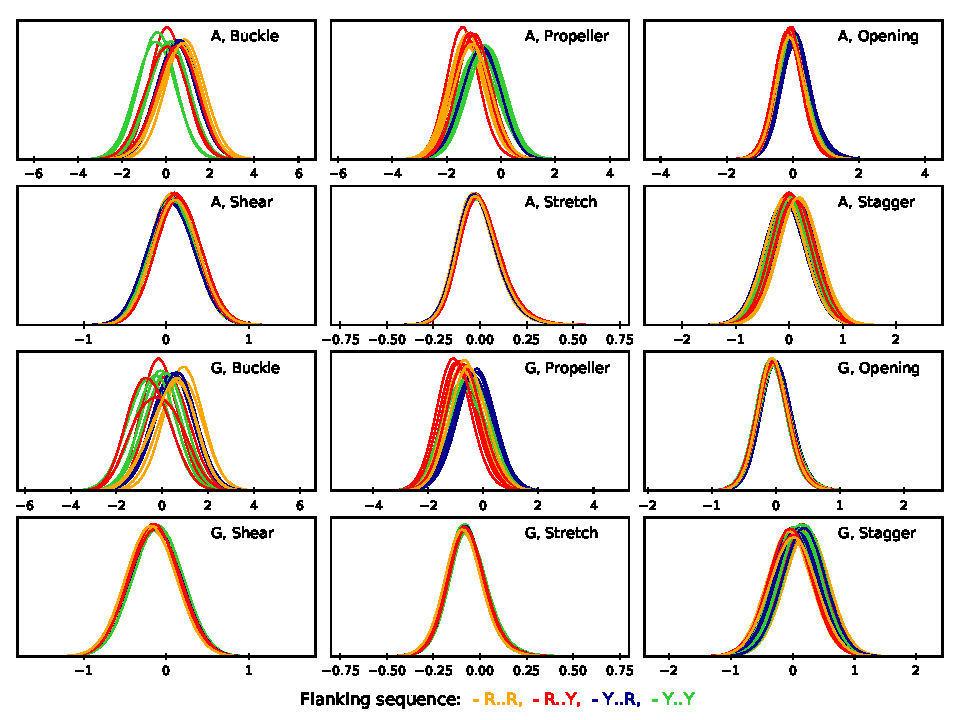
\includegraphics[width=15cm,trim=0cm 0cm 0cm 0.6cm]{images/DNA_intra_A_G.pdf}
    \caption{Intra base-pair coordinates in dsDNA}
  \end{subfigure}
  \begin{subfigure}{15cm}
    \centering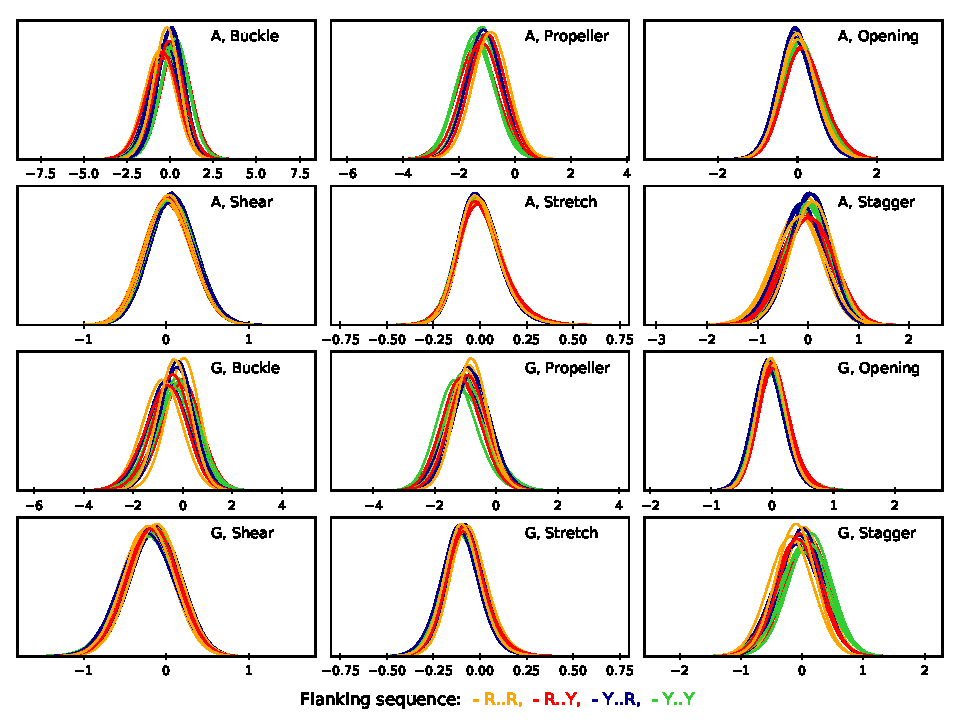
\includegraphics[width=15cm]{images/RNA_intra_A_G.pdf}
    \caption{Intra base-pair coordinates in dsRNA}
  \end{subfigure}
\caption{The normalized histograms for intra base-pair coordinates for A and G in all 16 trimer contexts in (a) dsDNA and (b) dsRNA as observed in MD time series of training sequences. The various contexts are plotted in different colors based on Y and R classification.  
}
\label{c3:fig_distr_1}
\end{figure} 

\begin{figure}[H]
  \begin{subfigure}{15cm}
    \centering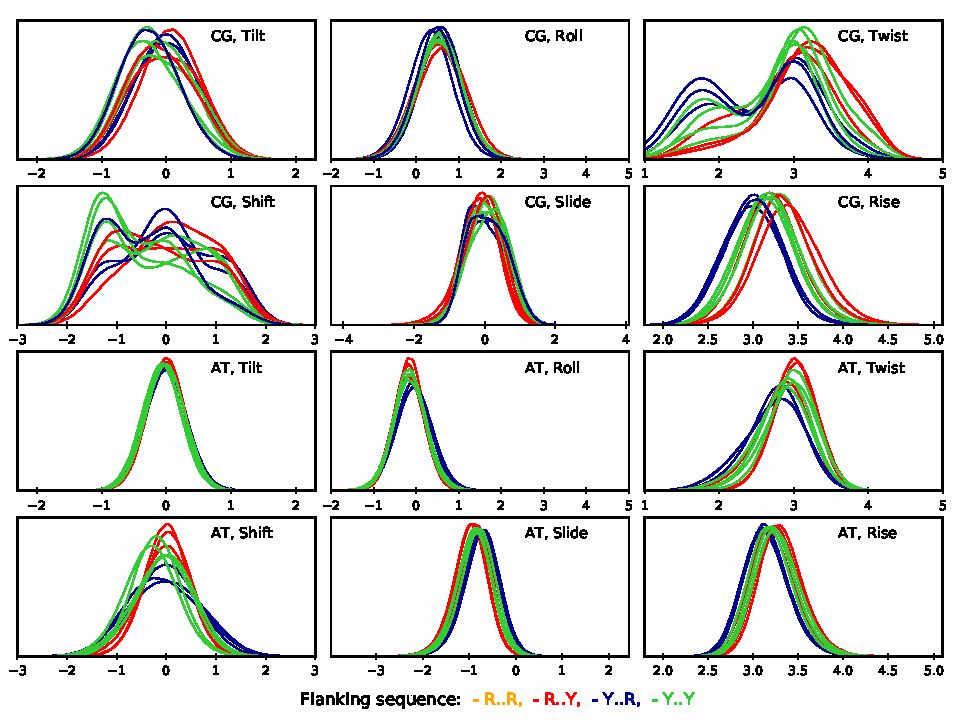
\includegraphics[width=15cm,trim=0cm 0cm 0cm 0.6cm]{images/DNA_inter_CG_AT.pdf}
    \caption{Inter base-pair step coordinates in dsDNA}
  \end{subfigure}
  \begin{subfigure}{15cm}
    \centering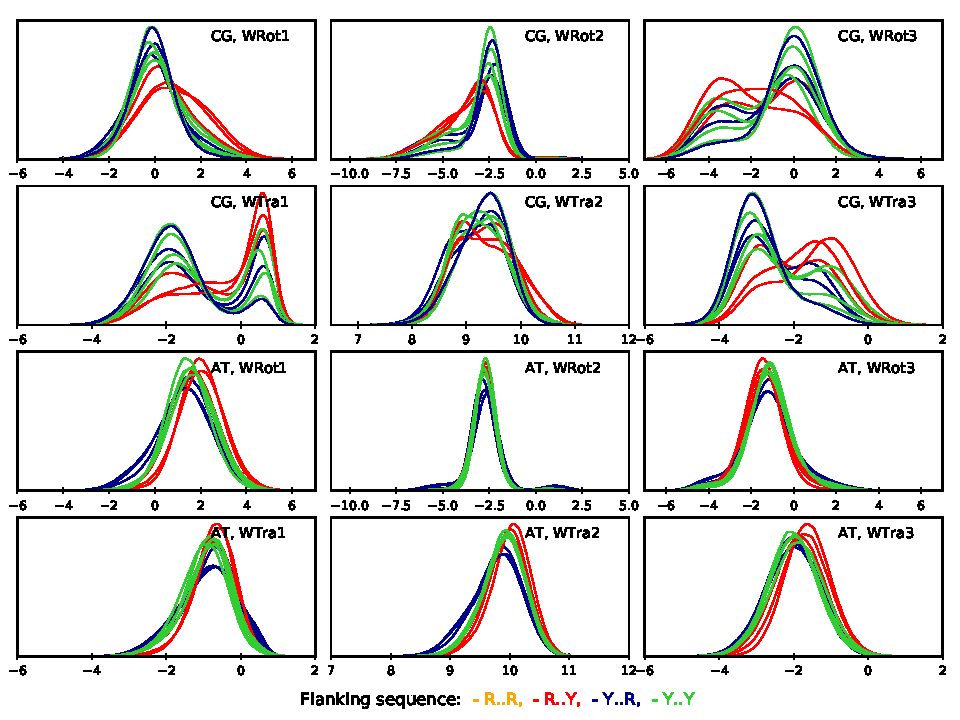
\includegraphics[width=15cm]{images/DNA_phosW_CG_AT.pdf}
    \caption{PhosW coordinates in dsDNA}
  \end{subfigure}
\caption{The normalized histograms for (a) inter base-pair step and (b) phosW coordinates for CG and AT in all 10 independent tetramer contexts for dsDNA observed in MD time series of the training sequences in \Lbdna. The various contexts are plotted in different colors based on Y and R classification.  
}
\label{c3:fig_distr_2}
\end{figure}


\begin{figure}[H]
  \begin{subfigure}{15cm}
    \centering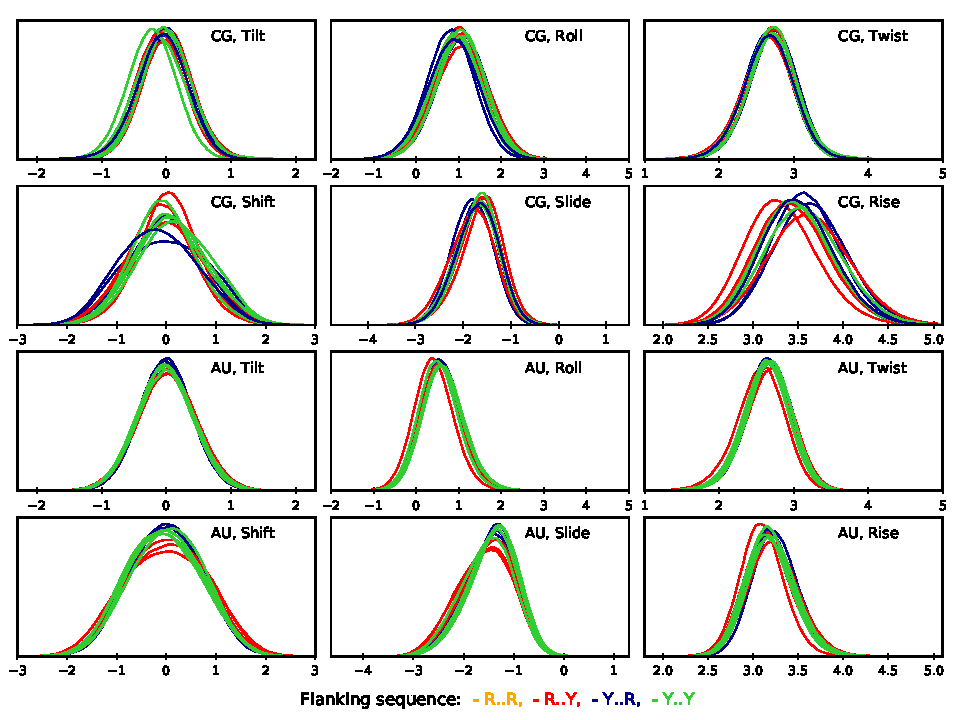
\includegraphics[width=15cm,trim=0cm 0cm 0cm 0.6cm]{images/RNA_inter_CG_AU.pdf}
    \caption{Inter base-pair step coordinates in dsRNA}
  \end{subfigure}
  \begin{subfigure}{15cm}
    \centering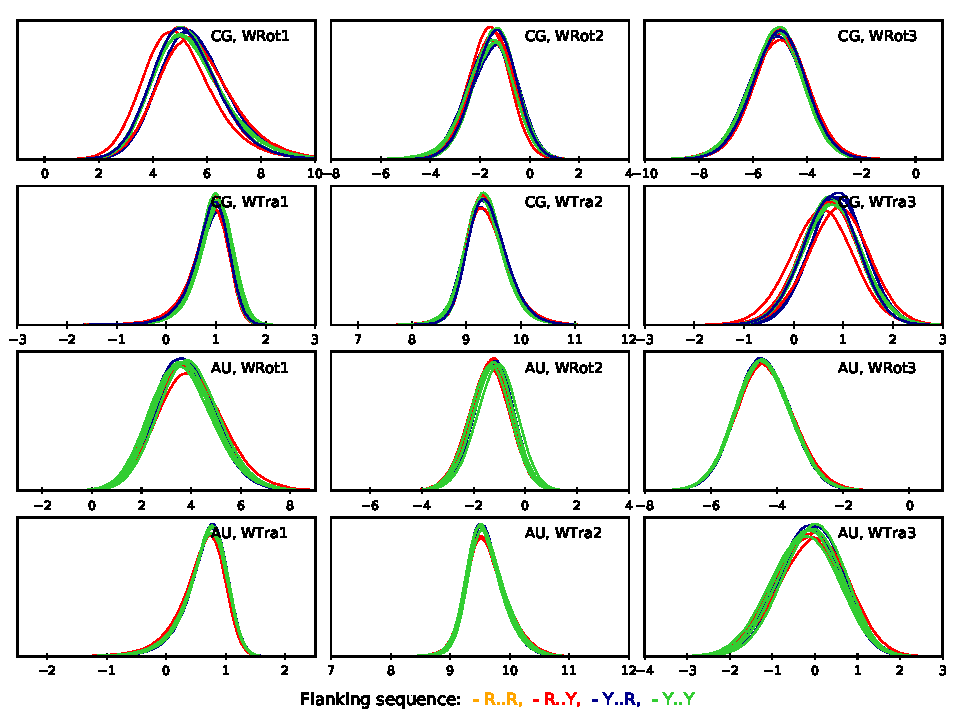
\includegraphics[width=15cm]{images/RNA_phosW_CG_AU.pdf}
    \caption{PhosW coordinates in dsRNA}
  \end{subfigure}
\caption{The normalized histograms for (a) inter base-pair step and (b) phosW coordinates for CG and AU in all 10 independent tetramer contexts for dsRNA observed in MD time series of all the training sequences in \Lbrna. The various contexts are plotted in different colors based on Y and R classification. 
}
\label{c3:fig_distr_3}
\end{figure}


\begin{figure}[H]
  \begin{subfigure}{15cm}
    \centering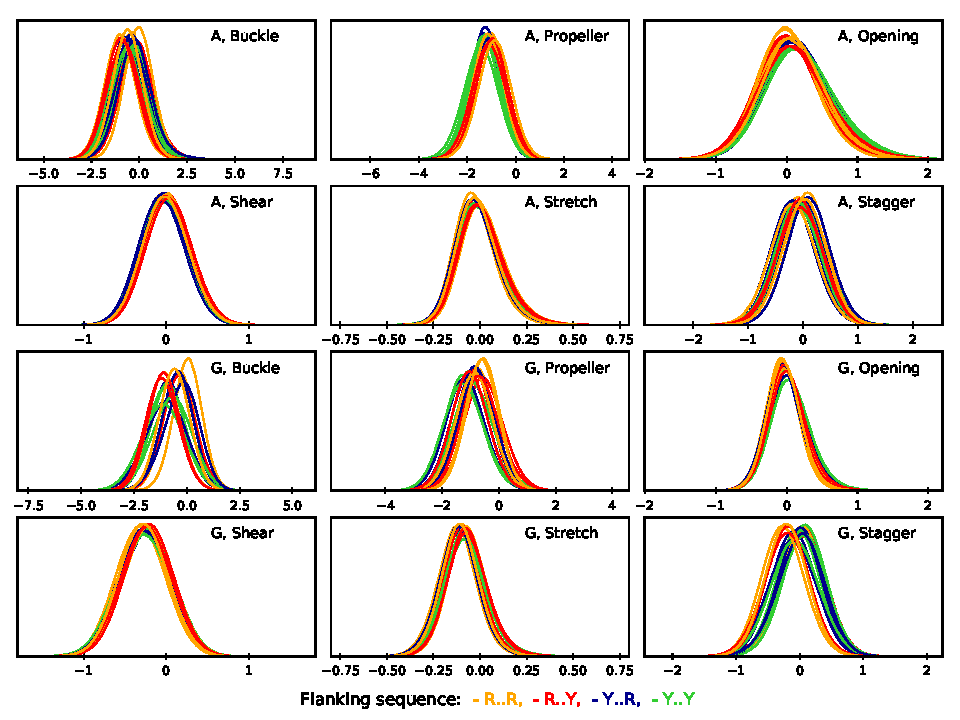
\includegraphics[width=15cm,trim=0cm 0cm 0cm 0.6cm]{images/HDR_intra_A_G.pdf}
    \caption{Intra base-pair coordinates in DRH}
  \end{subfigure}
  \begin{subfigure}{15cm}
    \centering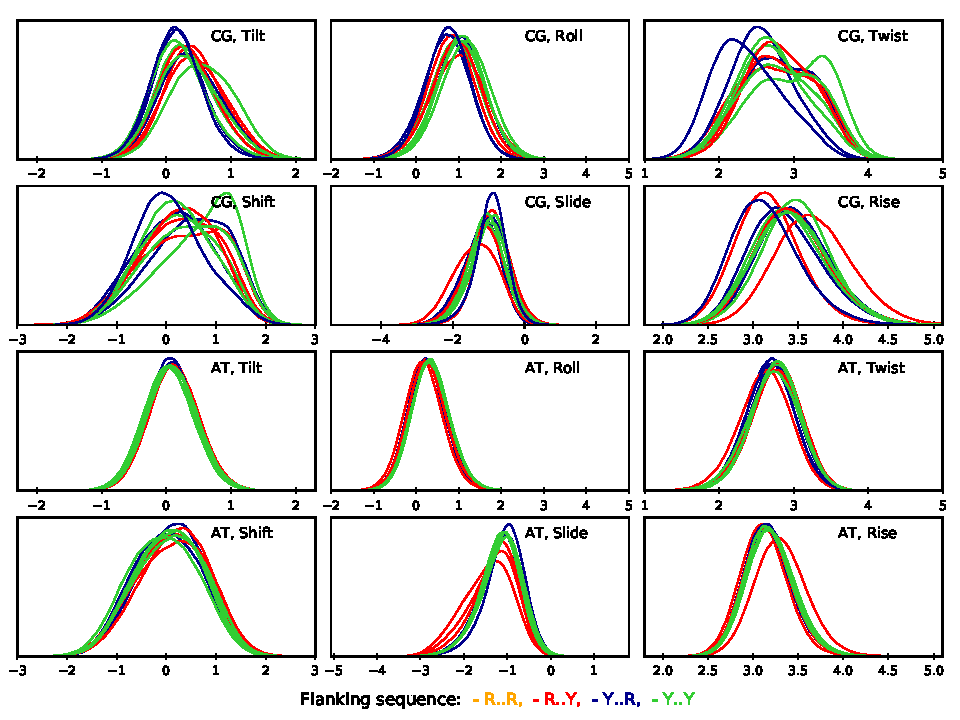
\includegraphics[width=15cm]{images/HDR_inter_CG_AU.pdf}
    \caption{Inter base-pair step coordinates in DRH}
  \end{subfigure}
\caption{The normalized histograms for (a) intra base-pair coordinates for A and G and (b) inter base-pair step coordinates CG and AT in all immediate flanking contexts for DRH observed in MD time series of all the training sequences in \Lbdrh. 
The various contexts are plotted in different colors based on Y and R classification. 
}
\label{c3:fig_distr_4}
\end{figure}

\section{Gaussian approximation error}\label{c3:s7}
In this final section, we have quantified the error associated with the Gaussian approximation of the model in the underlying distributions of the internal coordinates.
In \cref{c3:fig_hist_filter1,c3:fig_hist_filter2,c3:fig_hist_filter3,c3:fig_hist_filter4,c3:fig_distr_1,c3:fig_distr_2,c3:fig_distr_3,c3:fig_distr_4,c3:fig_distr_5}, we have shown that the observed distributions of internal coordinates in MD simulations often deviate from Gaussian behavior, in particular, phosphate coordinates and Shift, Slide, and Twist in the inter-coordinates.
Here, we have quantified the error, $\er_{\text{KL}}^{\text{Gauss}}$ corresponding to the assumption in the model that the internal coordinates follow Gaussian behavior by numerically computing symmetric KL divergence between the observed internal coordinate distribution in MD simulations and the corresponding best-fit Gaussian as defined in \cref{c2:s5sb22}.

In \cref{c3:fig_gauss_err}, we have plotted $\er_{\text{KL}}^{\text{Gauss}}$ for each internal coordinate of sequence index 1 in (a) \Lbdna, (b) \Lbrna, and (c) \Lbdrh \ as heat map with the sequence shown on the labels. 
The plots for the corresponding distributions for sequence index 1 in \Lbdna \ are shown in \cref{c3:fig_hist_filter1,c3:fig_hist_filter2,c3:fig_hist_filter3,c3:fig_hist_filter4} where it can be visually concluded that intra coordinates are close to Gaussian, some of the inter coordinates deviate from Gaussian behavior and almost all phosphate coordinates show non-Gaussian distributions.
The same observation can be confirmed quantitatively in terms of  $\er_{\text{KL}}^{\text{Gauss}}$ from \cref{c3:fig_gauss_err}(a) in which KL divergence between the observed distribution and corresponding best-fit Gaussian for intra coordinates is approximately 0.004 (average), for inter coordinates is 0.011 (average) and for Crick/Watson phosphate coordinates is 0.057 (average).
Notably, $\er_{\text{KL}}^{\text{Gauss}}$ for any particular internal coordinate, in general, depends on the dimer step (or monomer for intra coordinates) as well as on the flanking context.
For instance, $\er_{\text{KL}}^{\text{Gauss}}$ for Wtra1 for AG steps is much larger than any TT steps as well as $\er_{\text{KL}}^{\text{Gauss}}$ for AG steps at 5$^\text{th}$ or 22$^\text{nd}$ in different flanking contexts are considerably different.
In the same plot, one can also observe a Crick-Watson symmetry in inter/intra coordinates (the two half of the plots look similar) and in Crick and Watson phosphates (the two are similar when looked at from opposite directions).

In \cref{c3:fig_distr_3}, we have plotted the distributions for internal coordinates as observed in the MD simulations of training sequences in \Lbrna, highlighting that the distributions are very close to Gaussian behavior. 
In \cref{c3:fig_gauss_err}(b), we have shown the corresponding $\er_{\text{KL}}^{\text{Gauss}}$ in a heat map with similar conclusions. 
The average $\er_{\text{KL}}^{\text{Gauss}}$ is approximately 0.004, 0.003, and 0.019 in intra, inter, and phosphate coordinates, respectively.
The average $\er_{\text{KL}}^{\text{Gauss}}$ in intra coordinates are comparable for dsDNA and dsRNA. 
In contrast to dsDNA, the average $\er_{\text{KL}}^{\text{Gauss}}$ is considerably lower for dsRNA in inter and phosphate coordinates. 
Moreover, in \cref{c3:fig_gauss_err}(c), we have shown the corresponding $\er_{\text{KL}}^{\text{Gauss}}$ for sequence index 1 in \Lbdrh. 
Firstly, it can be noted that there is no Crick-Watson symmetry in phosphates, inter, or intra coordinates.
The average $\er_{\text{KL}}^{\text{Gauss}}$ in intra coordinates is approximately 0.005, which is comparable to the corresponding observations in dsDNA or dsRNA.
The corresponding error in inter coordinates is approximately 0.006 which is almost double than $\er_{\text{KL}}^{\text{Gauss}}$ for dsRNA (0.003) and half than $\er_{\text{KL}}^{\text{Gauss}}$ for dsRNA (0.011).
Lastly, the two phosphate coordinates (on Crick and Watson strands) in DRH, as shown in \cref{c3:fig_distr_5} behave differently depending on the strand type (DNA or RNA).
The average $\er_{\text{KL}}^{\text{Gauss}}$ for Crick phosphates (RNA strand) and Watson phosphates are approximately 0.036 and 0.029, which are comparable and closer to the observed values for dsRNA (0.019) than dsDNA (0.056).
However, note that Wtra1 is often multi-modal, in particular, for TG and GA steps. 

Thus, in this section, we have quantified the approximation error due to the Gaussianity imposition on the observed internal coordinates distributions in MD simulations.
One can visualize the magnitude of this error expressed in terms of the KL divergence using \cref{c2:KL_envelope}.
In general, we can conclude that for intras and most inters, the Gaussianity imposition is a natural choice. 
In contrast, for phosphate coordinates, $\er_{\text{KL}}^{\text{Gauss}}$ is considerable (average for dsDNA $\approx 0.057$) which goes as high as 0.459 for GA step as shown in \cref{c3:fig_gauss_err}(a).
For such cases, the Gaussianity imposition is questionable. 
Non-Gaussian models are certainly a better approach for treating such cases, but introduce several modeling challenges, e.g., a significant increase in model parameters and finding a parameter set in such high dimensions.
In this work, we have continued with the Gaussianity approximation, and non-Gaussian models are left for future research.
In principle, such a non-Gaussian model can be realized using quartic free-energy; however, the complexity of quartic models could easily explode for such large dimensions. 
A feasible compromise can be introducing sequence-independent non-Gaussian perturbation in the sequence-dependent Gaussian cgDNA$+$ model.
%Lastly, this non-Gaussian behavior of phosphate coordinates (which is also coupled with the inter coordinates) is related to NAs' backbone conformations as well as sugar pucker modes.
%Thus, 
%In \cref{c7}, we have introduced a 

\begin{figure}[H]
  \begin{subfigure}{15cm}
    \centering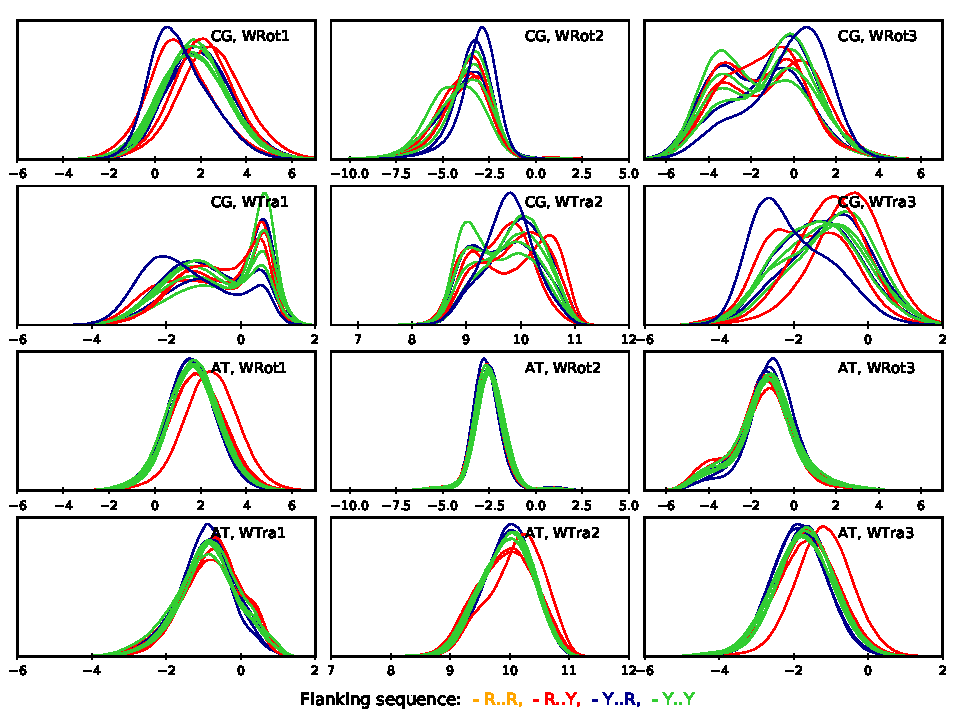
\includegraphics[width=15cm]{images/HDR_phosW_CG_AU.pdf}
    \caption{PhosW coordinates in DRH}
  \end{subfigure}
  \begin{subfigure}{15cm}
    \centering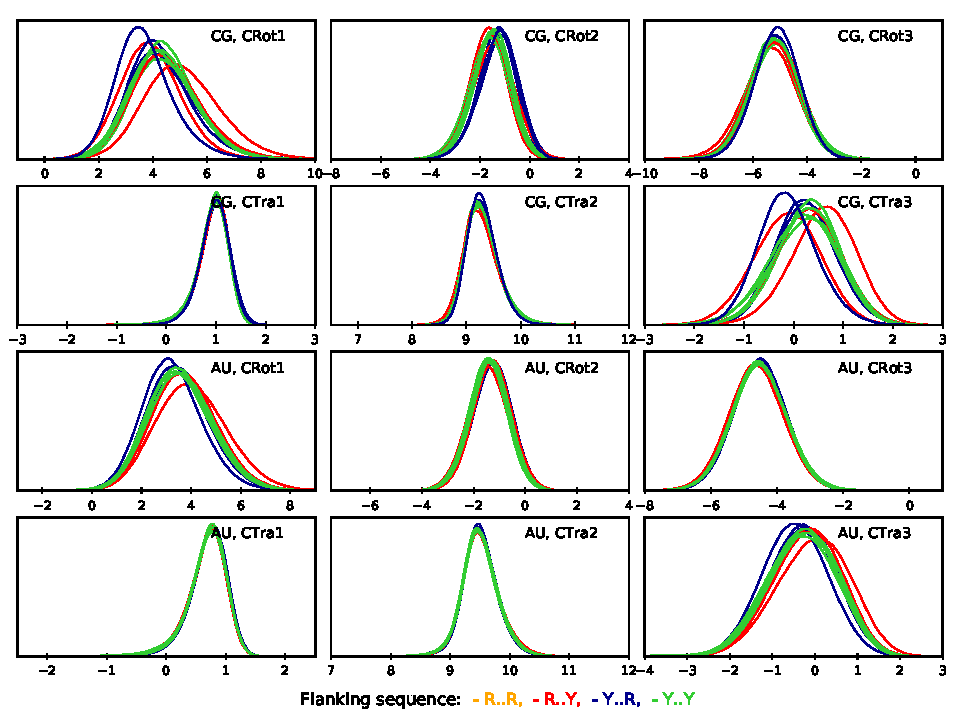
\includegraphics[width=15cm,trim=0cm 0cm 0cm 0.6cm]{images/HDR_phosC_CG_AU.pdf}
    \caption{PhosC coordinates in DRH}
  \end{subfigure}
\caption{
The normalized histograms for (a) phosW and (b) phosC coordinates for CG and AT/AU in all flanking tetramer contexts for DRH were observed in the MD time series of all the training sequences in \Lbdrh. The various contexts are plotted in different colors based on Y and R classification. 
}
\label{c3:fig_distr_5}
\end{figure} 

\begin{figure}[H]
  \begin{subfigure}{15cm}
    \centering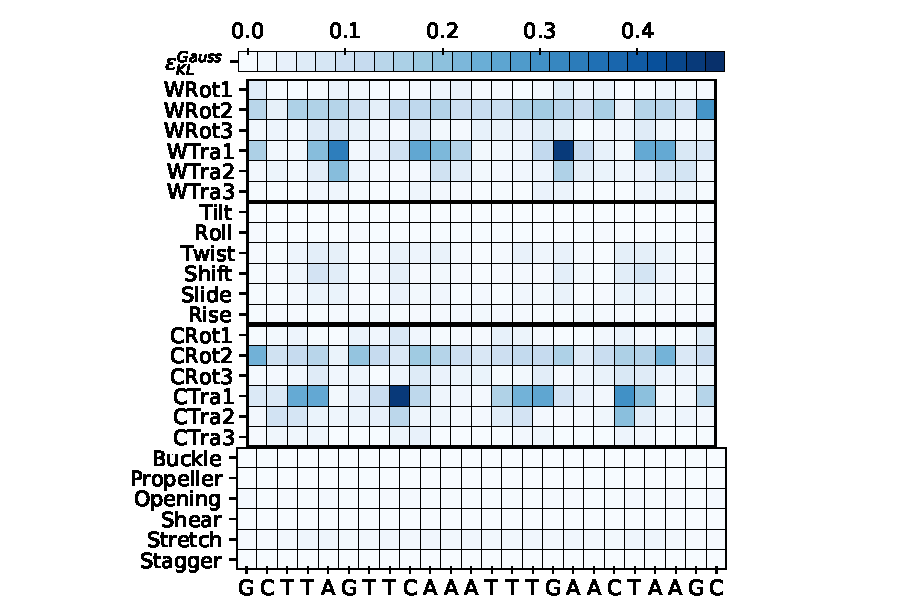
\includegraphics[width=11cm, trim=0cm 0cm 0cm 0.7cm]{images/Gaussian_error_DNA_1.pdf}
    \caption{$\er_{\text{KL}}^{\text{Gauss}}$ for sequence index 1 in \Lbdna}
  \end{subfigure}
  \begin{subfigure}{15cm}
    \centering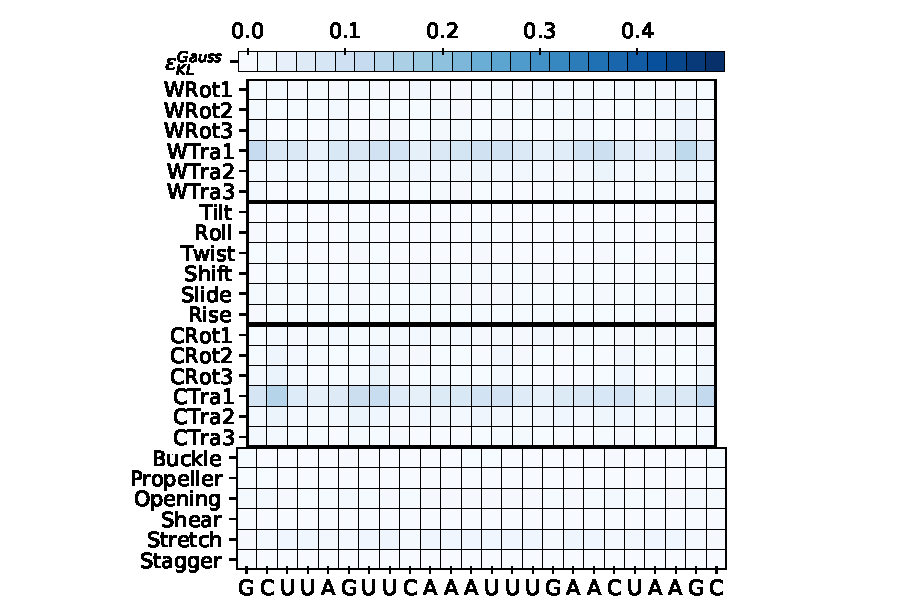
\includegraphics[width=11cm]{images/Gaussian_error_RNA_1.pdf}
    \caption{$\er_{\text{KL}}^{\text{Gauss}}$ for sequence index 1 in \Lbrna}
  \end{subfigure}
  \begin{subfigure}{15cm}
    \centering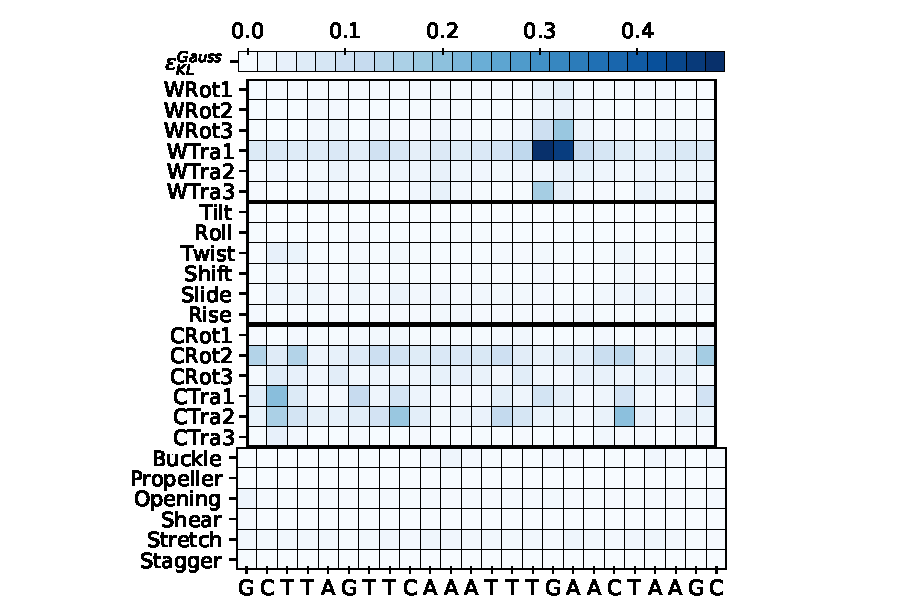
\includegraphics[width=11cm]{images/Gaussian_error_DRH_1.pdf}
    \caption{$\er_{\text{KL}}^{\text{Gauss}}$ for sequence index 1 in \Lbdrh}
  \end{subfigure}
\caption{
Gaussian approximation error, $\er_{\text{KL}}^{\text{Gauss}}$ in the internal coordinate distribution in MD simulations for sequence index 1 in (a) \Lbdna, (b) \Lbrna, and (c) \Lbdrh \ which is numerically computed as the symmetric KL divergence between the observed internal coordinate distribution in MD simulations and the corresponding best-fit Gaussian.
}
\label{c3:fig_gauss_err}
\end{figure} 
